\documentclass[11pt]{article}
\usepackage{amsfonts,amsmath,amssymb,amsthm}
\usepackage{graphicx,psfrag,epsf}
\usepackage{enumerate}
\usepackage{url} % not crucial - just used below for the URL
\usepackage{algorithm}
\usepackage{algpseudocode}
\usepackage{subfig}
\usepackage{authblk}
\usepackage{verbatim} %used to comment out unnecessary contents
\usepackage{helvet}
\usepackage[colorlinks=true,pagebackref,linkcolor=magenta]{hyperref}
\usepackage[sort&compress,comma,square,numbers]{natbib}
\usepackage{fullpage,fancyhdr}
\renewcommand{\familydefault}{\sfdefault}
\usepackage{color} %used to highlight changes
\usepackage{paralist}
\usepackage{lineno}
% \usepackage{todonotes}
\usepackage[font=footnotesize,labelfont=bf]{caption}
\usepackage[final,authormarkup=none]{changes}
\newcommand{\note}[2][]{\added[#1,remark={#2}]{}}
\definecolor{green}{rgb}{0.1840,0.4362,0.1003} 

\usepackage{tikz}
\usepackage{graphicx}
\usetikzlibrary{calc}
% \usepackage[nottoc,numbib]{tocbibind}
% \usepackage{flushend}

%better toc
% \usepackage{tocloft}
% \setlength\cftparskip{-1pt}
% \setlength\cftbeforesecskip{2pt}
% \setlength\cftaftertoctitleskip{4pt}

\pagestyle{fancy}
% \oddsidemargin=-0.5in
% \evensidemargin=-0.5in
\textwidth=6.5in
\headwidth=6.5in
\textheight=9.0in
\headheight=0.0pt
\topmargin=0.0in
\headsep=0.0in
\renewcommand{\headrulewidth}{0pt}

\setlength{\parindent}{0em}
\setlength{\parskip}{0.7em}

% % DON'T change margins - should be 1 inch all around.
% \addtolength{\oddsidemargin}{-.5in}%
% \addtolength{\evensidemargin}{-.5in}%
% \addtolength{\textwidth}{1in}%
% \addtolength{\textheight}{-.3in}%
% \addtolength{\topmargin}{-.8in}%

%\providecommageneralizednd{\sct}[1]{{\sc \texttt{#1}}}
\providecommand{\sct}[1]{{\normalfont\textsc{#1}}}
\providecommand{\mt}[1]{\widetilde{#1}}
\providecommand{\mb}[1]{\boldsymbol{#1}}
\providecommand{\mc}[1]{\mathcal{#1}}
\newcommand{\Real}{\mathbb{R}}
\newcommand{\G}{c}
\newcommand{\K}{\mathcal{K}}
\newcommand{\LL}{\mathcal{L}}
\newcommand{\Migraine}{\sct{Migraine}}
\newcommand{\mtg}{\sct{m2g}}
\newcommand{\T}{^{\ensuremath{\mathsf{T}}}}           % transpose
\newcommand{\Linefor}[2]{%
    \State \algorithmicfor\ {#1}\ \algorithmicdo\ {#2} \algorithmicend\ \algorithmicfor%
}
\newcommand{\Lineif}[2]{%
    \State \algorithmicif\ {#1}\ \algorithmicdo\ {#2} \algorithmicend\ \algorithmicif%
}\newcommand{\subfigimg}[3][,]{%
  \setbox1=\hbox{\includegraphics[#1]{#3}}% Store image in box
  \leavevmode\rlap{\usebox1}% Print image
  \rlap{\hspace*{12pt}\raisebox{\dimexpr\ht1-0\baselineskip}{#2}}% Print label
  \phantom{\usebox1}% Insert appropriate spcing
}

\newcommand{\Mgc}{\sct{Mgc}}
\newcommand{\Mgcp}{\sct{Mgc$_P$}}
\newcommand{\Mgcd}{\sct{Mgc$_D$}}
\newcommand{\Mgcm}{\sct{Mgc$_M$}}
\newcommand{\Hhg}{\sct{Hhg}}
\newcommand{\Dcorr}{\sct{Dcorr}}
\newcommand{\Mcorr}{\sct{Mcorr}}
\newcommand{\Mantel}{\sct{Mantel}}

\newcommand{\website}{\url{https://github.com/neurodata/MGC/}}

\newcommand{\jv}[1]{{\note{jv: #1}}}
\newcommand{\cs}[1]{{\note{cs: #1}}}

\newcommand{\mbx}{\ensuremath{\mb{x}}}
\newcommand{\mby}{\ensuremath{\mb{y}}}
\newcommand{\rto}{\leftarrow}
\newcommand{\argmax}{\operatornamewithlimits{argmax}}
\newcommand{\argmin}{\operatornamewithlimits{argmin}}

%environment
\newtheorem{thm}{Theorem}
\newtheorem{appThm}{Theorem}
\setcounter{appThm}{0}
\newtheorem{lem}{Lemma}
\newtheorem{appLem}{Lemma}
\setcounter{appLem}{0}
\newtheorem{cor}{Corollary}
\newtheorem*{defi*}{Properties}
\newtheorem{asn}{Assumption}
\newcommand*\mean[1]{\bar{#1}}

\renewcommand{\algorithmicrequire}{\textbf{Input:}}
\renewcommand{\algorithmicensure}{\textbf{Output:}}

\pagenumbering{arabic}
\linenumbers


\begin{document}

\def\spacingset#1{\renewcommand{\baselinestretch}%
{#1}\small\normalsize} \spacingset{1}

% \title{\bf Dependence Discovery from Multimodal Data via  Multiscale Generalized Correlation}
\title{\bf Discovering Relationships Across Disparate Data Modalities}
% Discovering Relationships Among Multiple Multifarious Datatypes 
% \title{\bf Revealing the Scales of Dependency Between Multiple Data Modalities}
 % Datasets via  Multiscale Generalized Correlation}
\author[1,2]{Cencheng Shen} %\thanks{cshen6@jhu.edu}}
\author[1,3]{Carey E. Priebe}% \thanks{cep@jhu.edu}}
\author[3,4,6]{Mauro Maggioni}%\thanks{mauro.maggioni@jhu.edu}}
\author[1,5,6,7]{Joshua T. Vogelstein\thanks{jovo@jhu.edu}}
\affil[1]{Center for Imaging Science, Johns Hopkins University}
\affil[2]{Department of Statistics, Temple University}
\affil[3]{Department of Applied Mathematics and Statistics, Johns Hopkins University}
\affil[4]{Department of Mathematics, Johns Hopkins University}
\affil[5]{Department of Biomedical Engineering and Institute for Computational Medicine, Johns Hopkins University}
\affil[6]{Institute for Data-Intensive Engineering \& Science, Johns Hopkins University}
\affil[7]{Institute for Computational Medicine, Johns Hopkins University}
\maketitle
%\pagestyle{empty}

% submitting to science, we get 320 for content
% total: 455, need to remove >100 lines, almost entirely from results.

% 125 lines; target = 64
% \section{Introduction}

% number of lines per caption
% 1: 20 
% 2: 6
% 3: 6
% 4: 6
% 5: 9
% 6: 2
% total: ~60

% \bigskip
\begin{abstract}
Discovering whether certain properties are associated with other properties is fundamental to all science.
% \jv{all of science seems limiting}
As the amount of data increases, it is becoming increasingly difficult and important to determine whether one property of the data (e.g., cloud density) is related to another (e.g., grass wetness).  Only If they are related does it make sense to further investigate the nature of the relationship. Unfortunately, reliably identifying relationships can be challenging, especially when the properties themselves are complex and the relationship is nonlinear and high-dimensional. Here, we describe a procedure,  Multiscale Generalized Correlation (\Mgc), that addresses these challenges. 
Our key insight is that if two properties are related, comparisons between measurements of similar pairs of the first property (e.g., two clouds of similar density) should be correlated with the comparisons between corresponding measurements of the second property (grass wetness under those clouds). We demonstrate the statistical and computational efficiency of \Mgc~in both simulations and theory.  We then apply it to detect the presence and nature of the relationships between brain activity and personality, brain shape and disorder, and  brain connectivity and creativity.  Finally, we demonstrate that \Mgc~does not suffer from the false positives that have plagued parametric methods.  Our open source implementation of \Mgc~is applicable to fundamental questions confronting science, government, finance, and many other disciplines. 
\end{abstract}

\noindent%
{\it Keywords: testing independence, distance correlation, k-nearest-neighbor, kernel test, permutation test}
% \vfill

\clearpage
\setcounter{tocdepth}{2}% paragraphs and above
% {\small\tableofcontents}
% \addtocontents{toc}{\vspace{-3\baselineskip}}
% \listofchanges[style=list]

% \newpage
% \spacingset{1.45}

Identifying the existence of a relationship is a precursor to investigating the structure of the relationship,  whether it has predictive power, and whether it reflects causality.
One of the first statistical approaches to determine whether two properties are related to---or statistically dependent on---one another is Pearson's Product-Moment Correlation (published in 1895 \cite{Pearson1895}). This seminal advance   prompted the development of  entirely new ways of thinking about and quantifying relationships (see \cite{Reimherr2013,JosseHolmes2013} for  recent reviews and discussion).


Modern datasets, however, present particularly vexing challenges for dependence-testing, that were not foreseen in Pearson's era.
%
First, the \textbf{dimensionality} of individual samples is growing at exponential rates, with genomics and connectomics datasets, for example, often encompassing millions or even billions of dimensions. 
Second, the data are often \textbf{structured}---sequences, images, networks, shapes, and text---creating problems for standard methods that were developed for unstructured feature sets.
%
Third, the \textbf{sample sizes} are not increasing proportionally, meaning that we are often confronted with ultrahigh-dimensional datasets derived from relatively few samples.
% 
Fourth, the dependencies between different properties 
of data can be highly \textbf{nonlinear}, posing additional obstacles for the analysis of very large datasets.
%
Fifth, because of the continuing data deluge,  \textbf{computationally efficient} methods for analysis are critical for generating results within acceptable time frames
%
And finally, we not only want to know \textit{whether}  properties are dependent on each other, but also \textit{how} they are related.
There is thus a  need for methods that satisfactorily address all of these challenges and is supported by compelling evidence for its theoretical efficacy and practical utility.
% \jv{"and is" doesn't seem right above}

We developed the Multiscale Generalized Correlation (\Mgc) test to address those needs.
The key intuition behind  \Mgc~is illustrated in Figure \ref{f:schematic} using a canonical nonlinear  function: a spiral.  
\Mgc, like all tests for dependence, starts with observing $n$ samples, $(\mbx_i,\mby_i)$. 
While for linear functions, if a pair of samples are close in $x$ they will also be close in $y$, this is not always true for nonlinear functions.
In this specific example, points $1$ and $2$ are close in both $x$ and $y$, whereas points $2$ and $3$ are close only in $y$ and not $x$.
Thus, if one desires to determine whether $x$ and $y$ are in fact dependent on one another, 
restricting the analysis to the pairs that are close in both $x$ and $y$---the \emph{jointly local pairs}---rather than all pairs, could yield dramatic improvements.  
\Mgc~achieves this by identifying the jointly local pairs, 
and then using restricting its test to only those scales, thereby revealing both the existence and scales of dependence.
%
% A primary challenge that we faced was the determination the optimal local scales in a computationally efficient and statistically consistent manner. We constructed a five step approach to address this challenge. 
% \jv{the past paragraph ended with a challenge, and so does this one. seems like maybe another word would be ideal here.}
Given the above intuition, the remaining challenge was to ensure that \Mgc~could estimate the  optimal local scales in a computationally efficient and statistically consistent manner. We constructed a five step approach to address this challenge.


\begin{figure}[htbp]
\vspace{-50pt}
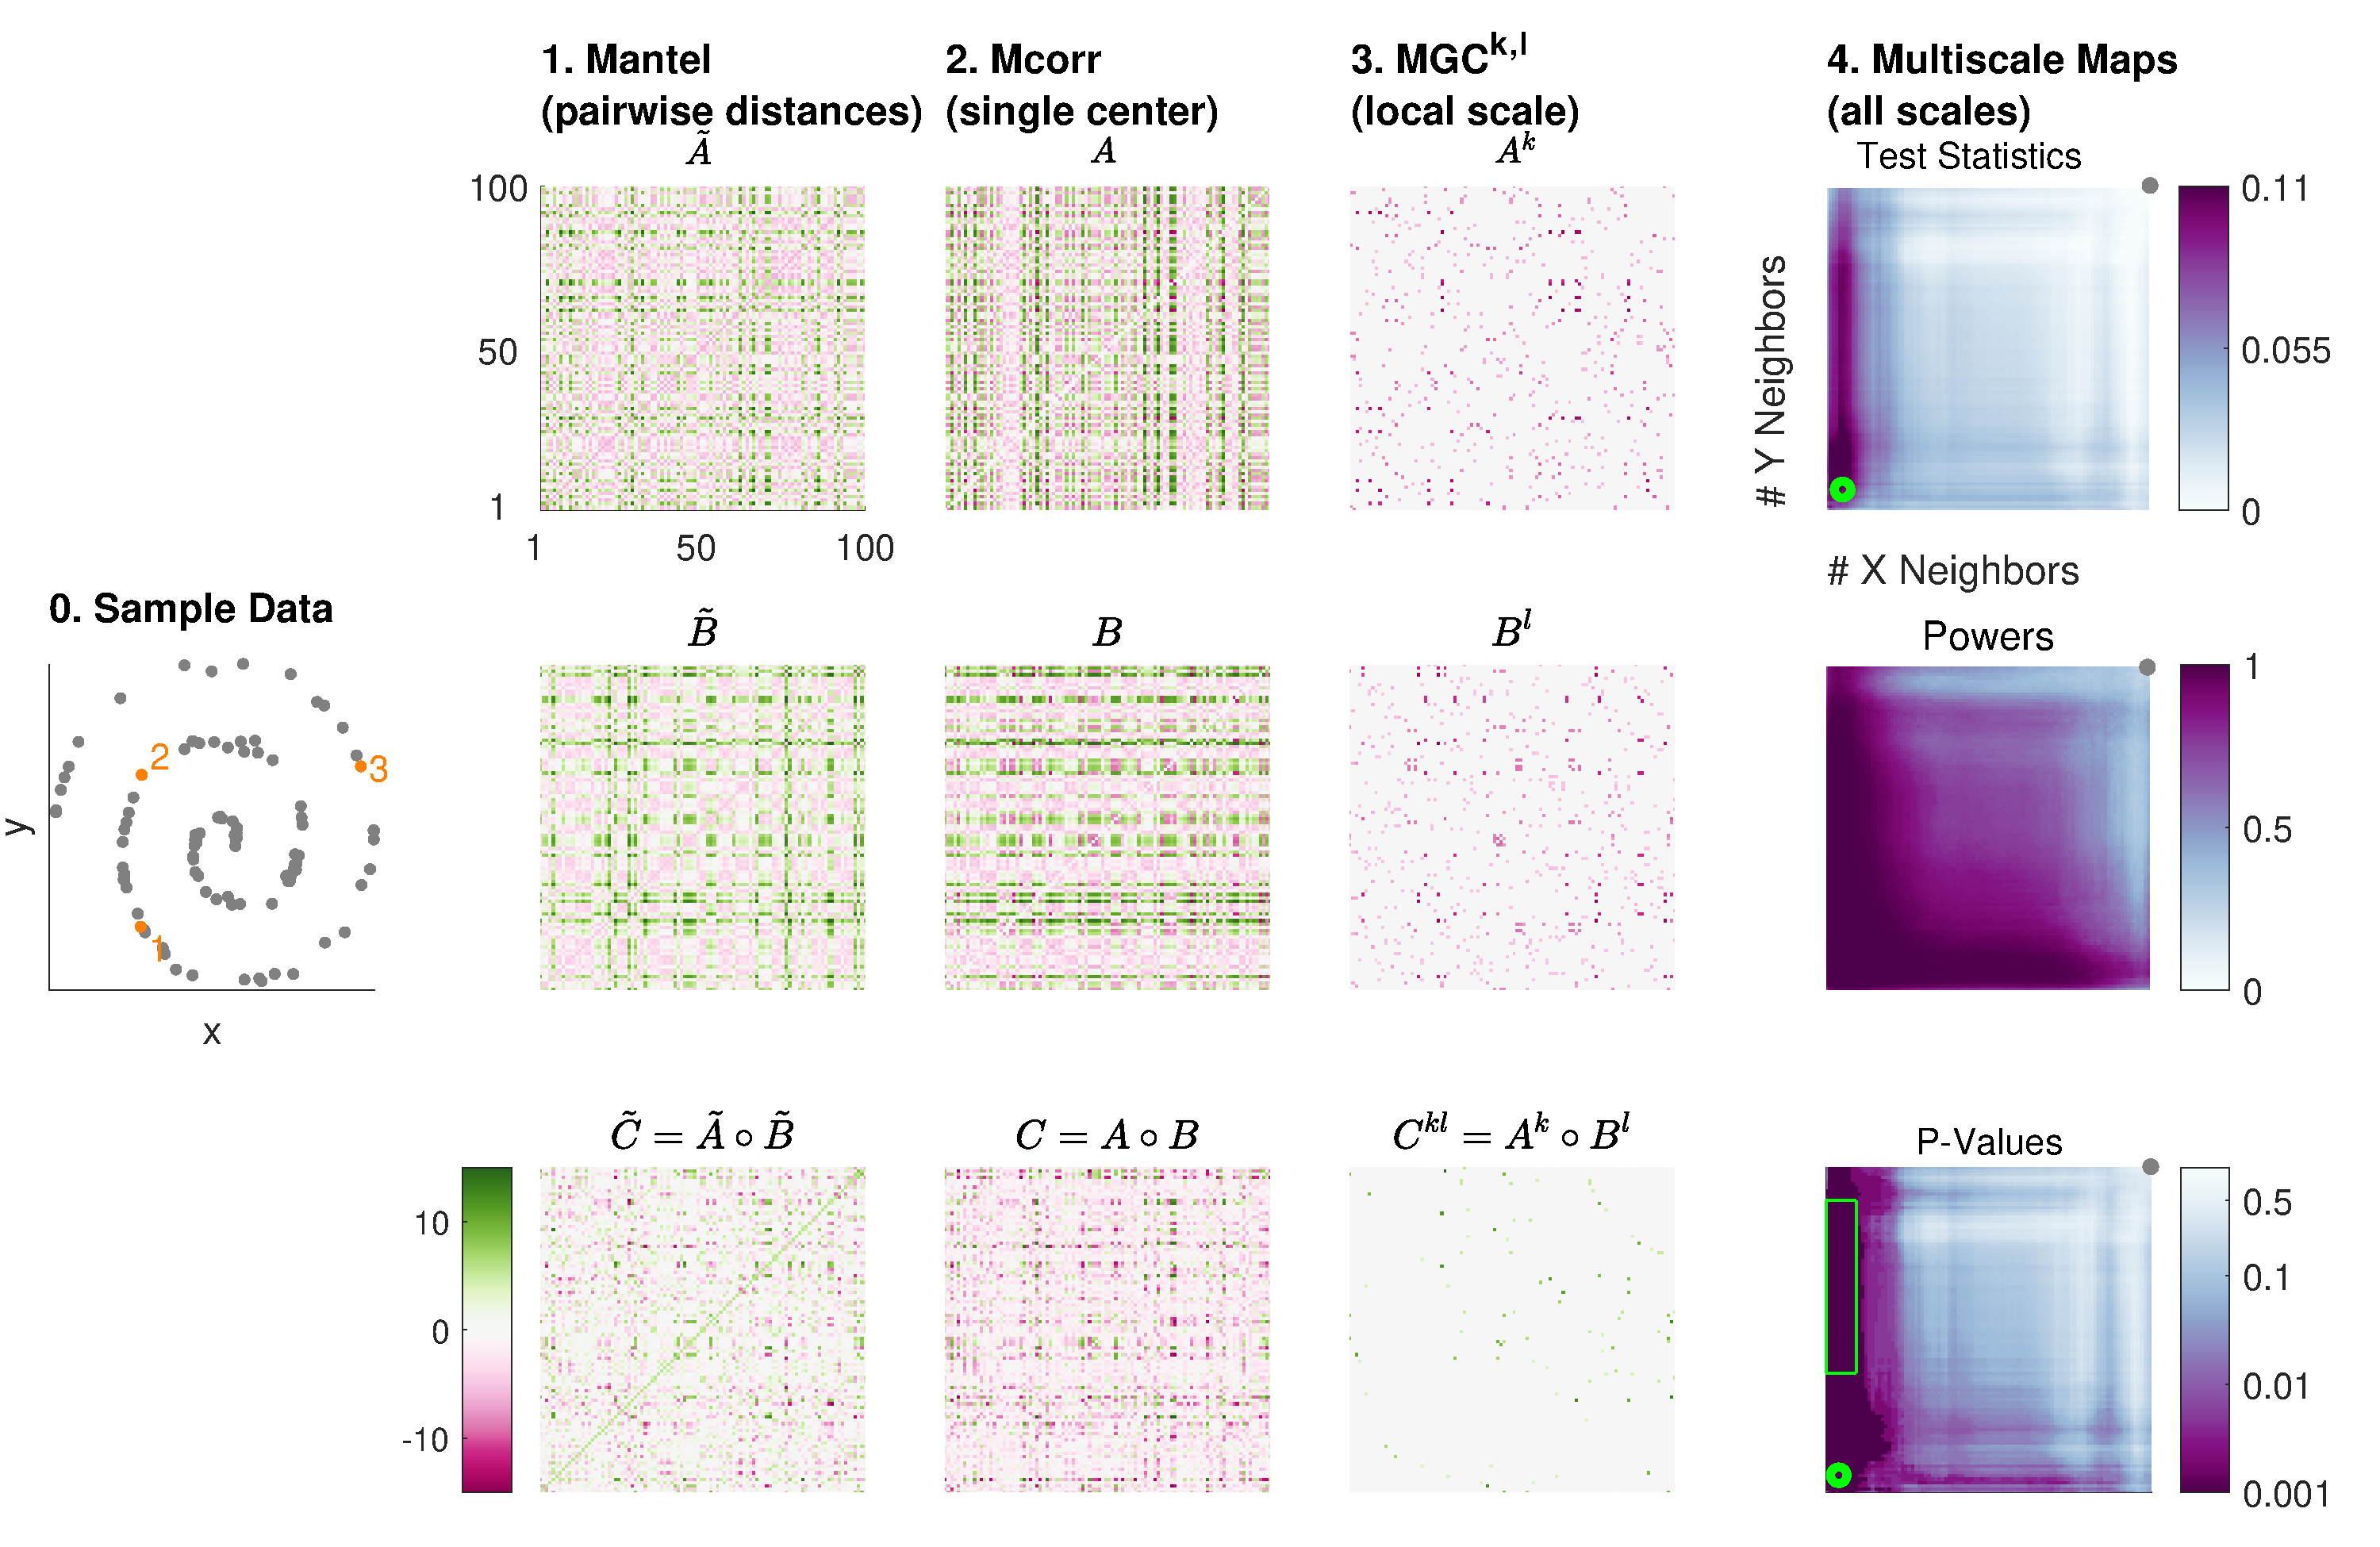
\includegraphics[width=1.0\textwidth,trim={0 0 2cm 0},clip]{Figures/FigA}
\setlength{\tabcolsep}{10pt} % Default value: 6pt
\begin{tabular}{r r r r}
\multicolumn{1}{l}{{\small \textbf{6. Table}}} & & & \\
$\delta_x$(1,2)   & \hspace{1.5em} \color{magenta}-1.75  & \hspace{3.5em} \color{magenta}-2.66  &  \hspace{3.0em} \color{magenta}-2.66  \\ 
 $\delta_y$(1,2) & \color{magenta}-2.00 & \color{magenta}-2.27 & \color{magenta}-2.27  \\ 
 $\delta_x \times \delta_y$ & \color{green}3.51 & \color{green}6.05 & \color{green}6.05  \\ 
 
\hline

 $\delta_x$(2,3) & \color{green}4.48 & \color{green}3.45 & 0.00  \\ 
 $\delta_y$(2,3) &  \color{magenta}-0.86 & \color{magenta}-0.26 & 0.00  \\ 
 $\delta_x \times \delta_y$ & \color{magenta}-3.87 & \color{magenta}-0.88 & 0.00  \\ 

\hline
 $\sum{\delta_x \times \delta_y}$ & \color{magenta}-147.18   & \color{green}7.06 & \color{green}159.72  \\ 
 test statistic &  \color{magenta}-0.02  & 0.00 & \color{green}0.24  \\  
\end{tabular}

\begin{tikzpicture}[remember picture,overlay]
\node[xshift=-5.2cm,yshift=-0.6cm] at (current page.east){%
    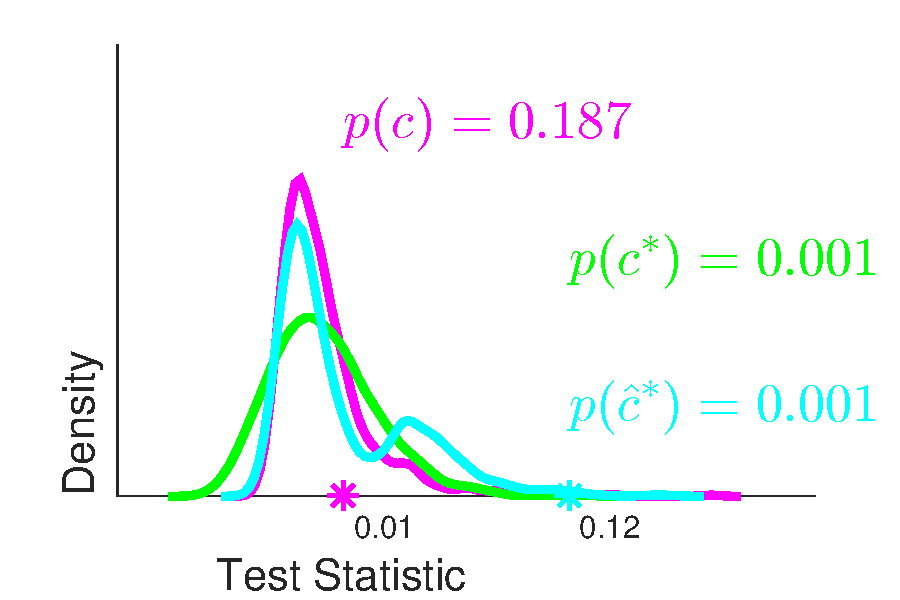
\includegraphics[width=0.35\textwidth,trim={1.5cm 0 1.8cm 0},clip]{Figures/FigB}};
  %\node[anchor=east,inner sep=0pt] at ($(current page.east)-(10cm,10cm)$) {
   %  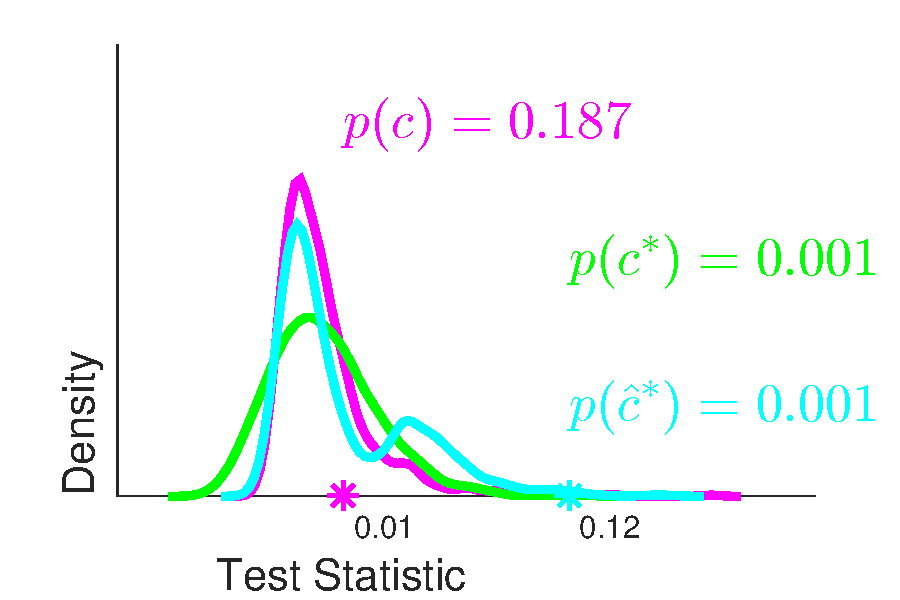
\includegraphics[width=0.3\textwidth]{Figures/FigB}
  %};
\end{tikzpicture}
\caption{
Flowchart  and table demonstrating the ability of Multiscale Generalized Correlation (\Mgc) to detect dependence in nonlinear settings. 
\textbf{0.} 50 pairs of observations $(x_i,y_i)$ are nonlinearly (spirally) dependent on one another.
% 
\textbf{1.} Choose a metric on $x$ and another on $y$, and compute all pairwise distances (centered by the overall means) for $x$ and $y$ yielding interpoint comparison matrices
 $\tilde{A}$ (top) and $\tilde{B}$ (middle), 
and their element-wise products $\tilde{C}=\tilde{A} \circ \tilde{B}$ (bottom), whose normalized sum is the  \Mantel~statistic \cite{Mantel1967} (bottom row of table).
% 
\textbf{2.} Single centering --- subtract the row-sums from $\tilde{A}$ and column-sums from $\tilde{B}$ to eliminate bias due to individual samples --- yields $A=\{a_{ij}\}$ and $B=\{b_{ij}\}$; the normalized sum of their  element-wise product  $C$ is equivalent to the  \Mcorr~statistic \cite{SzekelyRizzo2013a}.
% 
\textbf{3.} Given a local scale, for example, $k=l=4$ here, yields $A^{k}$, $B^{l}$, and $C^{kl}$.  Because all these test statistics are normalized sums of the element-wise products, the fact that \Mgc~yields a $C^{kl}$ matrix that is all positive, whereas the others yield $C$ matrices with both positive and negative values, suggest that \Mgc~will correctly report a large test statistic here, resulting in a small p-value.
\textbf{4.} Compute the test statistics (top), power (middle), and p-value (bottom) for all local scales, resulting in multiscale maps that reveal the  scales of dependency. 
\textbf{5.} Report the corresponding observed test statistics and p-values, and discover the optimal scales (green rectangle in  p-value map) by sample \Mgc.  
Whereas \Mcorr, the global test, has very low power (magenta dot in  p-value map) and therefore yields a small statistic and a non-significant p-value ($0.348$),  there are many local scales that achieve nearly perfect power, so both Oracle and sample \Mgc~($\G^{*}$ and $\hat{\G}^{*}$) obtain large test statistics and highly significant p-values ($\approx 0.001$) and reveal the scales of dependency. 
\textbf{6.} Numerical demonstration of how \Mgc~is able to detect dependence even in highly nonlinear and low-sample size settings. The three colored points in the scatter plot indicate the three points considered in this table. 
The global methods fail to detect significant dependence since they consider all pairs, including the non-local ones, which \emph{negatively} impact the degree of dependence estimated.
\Mgc~only considers pairs that are jointly local (such as $(1,2)$), while discarding other pairs (such as $(2,3)$). 
}
\label{f:schematic}
\end{figure}
 
The first step is to compute distances between all pairs of points \emph{within} each modality. Previous work demonstrated that  interpoint comparison matrices are actually sufficient for testing dependencies \cite{Maa1996} (which is closely related to theoretical results in the kernel machine literature \cite{scholkopf2002learning}). 
While data from disparate modalities are fundamentally incommensurate, by transforming the original data into pairwise distances, comparisons across data become meaningful.
More formally, let $\delta_x$ be the distance for $\mbx$ and $\delta_y$ for $\mb{y}$, and compute the $n \times n$ interpoint comparison matrices $A=\{a_{ij}\}$ and $B=\{b_{ij}\}$, where $a_{ij}=\delta_x(\mb{x}_i,\mb{x}_j)$ and  $b_{ij}=\delta_y(\mb{y}_i,\mb{y}_j)$.  
This ``generalized correlation coefficient''  \cite{Spearman1904,Mantel1967,KendallBook}, assuming $A$ and $B$ have zero mean without loss of generality, is written:
\begin{equation}
\label{generalCoef}
\G= \tfrac{1}{z} {\textstyle \sum_{i,j=1}^n a_{ij} b_{ij}},
\end{equation}
where $z$ is proportional to the standard deviations of $A$ and $B$, that is $z=n^2\sigma_a \sigma_b$.
In words, $\G$ is the global correlation across \emph{pairwise comparison matrices} $A$ and $B$, rather than the individual data samples.\footnote{Note that with this definition $\G$ is scale  invariant --- that is, if $\delta_x$ are $\delta_y$ are each multiplied by some factor (e.g. corresponding to using a different unit of measure in each variable), $\G$ is unchanged.} 
For all of these tests, and those that follow, given the test statistic, one can conduct a permutation test to obtain the p-value \cite{GoodPermutationBook}.

The second step is to ``single-center'' these matrices to ensure that each data point counts equally; without such centering, single data points far from the others could distort the statistics.
A celebrated body of  work collectively called \emph{energy statistics} \cite{RizzoSzekely2016} has shown that by doubly centering $A$ and $B$, one obtains a consistent test in a wide variety of settings.  
More formally, Szekely et al. (2007) \cite{SzekelyRizzoBakirov2007} proved that when  $\delta_x$ and $\delta_y$  are  Euclidean distances, if one subtracts the row and column means of $A$ and $B$ prior to taking their element-wise products and summing, the resulting test achieves optimal power as 
sample size approaches infinity, for any joint distribution of finite dimension and finite second moments. 
This distance correlation (\Dcorr) test essentially rescales each point to ensure that all sample points contribute equally to the dependence statistic. 
Szekely et al. \cite{SzekelyRizzo2013a} further proposed a modified version that we call \Mcorr, which they prove to be unbiased as the dimensions of $\mb{x}$ and $\mb{y}$ increase to infinity, thus consistent for high-dimensional dependencies as well.
We extend this result by proving that single centering --- subtracting the row means from $A$ and the column means from $B$ --- does not change the test statistic (see Lemma \ref{lem1} in Appendix \ref{appen:methods}), and simplifies the subsequent steps.
Because these distance-based tests merely require a distance function for both $X$ and $Y$, Lyons was able to prove that they are consistent even in general metric spaces satisfying certain properties, including certain networks, shapes, and other structured spaces  \cite{Lyons2013}.
Thus, existing tests  work well asymptotically for nonlinear and high-dimensional data,  including structured domains. 


Empirically, however, distance correlation tests struggle in various nonlinear and high-dimensional settings. We conjectured that their struggles in finite-sample testing were due to the fact that they were \emph{global methods}, and therefore they consider all pairs of points, including non-local ones. They also cannot provide insight into the scales of the dependence. We therefore adopted the locality principle, which has reaped considerable benefits in a wide range of data science problems, including  classification and regression  \cite{Stone1977}, data compression \cite{DaubechiesWaveletBook}, and recommender systems \cite{Sarwar2000}.
Moreover, it has become an invaluable tool in unfolding nonlinear geometry in many nonlinear dimensionality reduction (or manifold learning) algorithms (for example, \cite{
TorgersonBook, 
TenenbaumSilvaLangford2000, 
SaulRoweis2000, 
BelkinNiyogi2003,
DiffusionPNAS,
MMS:NoisyDictionaryLearning}). 
However, only a few papers have utilized locality for testing purposes \cite{David1966,Friedman1983,Schilling1986}.  These tests, like the ones based on distance correlation, have the advantage of naturally operating on complicated data, because they only require a comparison function between observations.  They can also have strong theoretical guarantees \cite{Maa1996}, but they are for testing equality of distribution for data from the same modality, and we are interested in testing for dependence across different modalities. 

To endow \Mgc~with the ability to utilize locality, 
the third step is to compute a local variant of the distance correlation test.
To obtain a local dependence test, 
\Mgc~sorts the distance matrices based on locality.
To do so, \Mgc~computes the ``rank'' of each pairwise distance: 
let $R(a_{ij})$  be the ``rank'' of $\mb{x}_i$ relative to $\mb{x}_j$, that is, $R(a_{ij})=k$ if $\mb{x}_i$ is the $k^{th}$ closest point (or ``neighbor'') to $\mb{x}_j$, and define $R(b_{ij})$ equivalently for the \mby's. For any neighborhood size $k$ around each $\mb{x}_i$~and any neighborhood size $l$ around each $\mb{y}_i$, we define the local pairwise comparisons:
\begin{equation}
\label{localCoef2}
    \mt{a}_{ij}^k=
    \begin{cases}
      a_{ij}, & \text{if } R(a_{ij}) \leq k, \\
       % -\bar{a}^{k}, & \text{otherwise};      
      0, & \text{otherwise};
    \end{cases} \qquad \qquad
    \mt{b}_{ij}^l=
    \begin{cases}
      b_{ij}, & \text{if } R(b_{ji}) \leq l, \\
       % -\bar{b}^{l}, & \text{otherwise};
      0, & \text{otherwise};
    \end{cases}
\end{equation}
and then let $a^k_{ij}=\mt{a}^k_{ij} - \bar{a}^k$, 
where $\bar{a}^k$ is the local mean. Then, define $b^k_{ij}$ similarly, except the rank index is transposed. 
The \emph{local} variant of any global generalized correlation coefficient therefore  excludes large distances: % up-to the centering scalars:
\begin{equation}
\label{localCoef}
\G^{kl}=\dfrac{1}{z_{kl}} {\textstyle \sum_{i,j=1}^n a_{ij}^k b_{ij}^l},
\end{equation}
where $z_{kl}=n^2 \sigma_a^k \sigma_b^l$,  with $\sigma_a^k$ and $\sigma_b^{l}$ being the standard deviations for the truncated pairwise comparisons. Thus, $c^{kl}$ is the local test statistic, for a given scale.


\Mgc~can be thought of as a sparse or regularized variant of a global correlation test, and therefore it faces the same dilemma as all regularized algorithms (including sparse methods, feature selection, and dimension reduction): how to efficiently choose the parameters. By choosing the locality scales in a principled fashion, \Mgc~both yields a consistent test and reveals the scales of dependence.  
Many manifold learning algorithms require that the user essentially runs the entire algorithm again from scratch for each different parameter setting, a pursuit that can be exponentially taxing as the number of parameters increases.  
Since there are $n^2$ different local tests, one for each possible combination of $k$ and $l$, the challenge is to find a way to compute all local tests in a computationally efficient fashion. 


The fourth step is therefore to compute all local tests in a nested algorithm, re-using adjacent smaller local correlations to procedurally build all local statistics, and efficiently yielding multiscale maps that reveal the scales of dependence. 
For a given scale, once the rank information is provided, the local correlation takes $O(n^2)$ time to compute (because it requires calculating a distance for all pairs; see Algorithm \ref{alg:1scale}). 
% 
However, doing so na\"ively for each scale separately requires $O(n^4)$ time, because there are $O(n^2)$ different scales to consider. 
% 
By noting that the sufficient statistics for larger neighborhood sizes include those for the smaller sizes, one can simply keep track of the sufficient statistics while iteratively increasing neighborhood size, yielding  \emph{all} local correlations in $O(n^2 \log n)$, essentially the same running time complexity as  global correlation coefficients (Algorithms \ref{alg:all_scales}). Specifically, \Mantel, \Dcorr, and \Mcorr~require $O(n^2)$ time, and \Hhg, another state-of-the-art approach,  requires $O(n^2 \log n)$ time \cite{HellerGorfine2013}.  Upon computing the test statistics for all scales, \Mgc~yields ``multiscale maps'', which it then uses to estimate the optimal scale.\footnote{These maps are  related to, but quite distinct from, maps of wavelet coefficients commonly used in geometric counterparts of harmonic analysis \cite{Allard2012,MMS:NoisyDictionaryLearning}.}


The fifth step is to compute the p-value and optimal scales.
We define the optimal scales for a given distribution and number of samples as the scales that maximize power (the probability of correctly rejecting a false null hypothesis).  
``Oracle \Mgc'' chooses the optimal scales by simulating from an assumed or estimated distribution with a given sample size and selecting the scales that maximize power  (Algorithm \ref{alg:power}).
In real data without sufficient training data, the true distribution is unavailable so we cannot compute the power to calculate the optimal scales or the optimal test statistic.
We therefore designed  ``sample \Mgc'' to estimate  them without relying on the power map. 
From the multiscale test statistic map, sample \Mgc~finds the region with the largest test statistic (ignoring sparse noisy scales, Algorithm \ref{alg:sample_mgc}).  The p-value of sample \Mgc, $p(\hat{c}^*)$, follows from a permutation test using the estimated optimal statistic within that region.
To determine the optimal scales, we find the tightest bounding box around all local scales with a p-value equal to or lower than $p(\hat{c}^*)$ (Algorithm \ref{alg:pval}).
Because neither the Oracle \Mgc~nor sample \Mgc~compares multiple statistics, neither suffers from the multiple hypothesis testing problem \cite{Benjamini1995}.

The table in Figure \ref{f:schematic} illustrates how \Mgc~is able to detect dependence, even in this spiral example with only $50$ samples, while the global correlation tests fail.  Samples $1$ and $2$ are close to each other in both $x$ and $y$; they therefore contribute to \emph{positive} dependence for all three tests.  However, samples $2$ and $3$ are only close in $x$, not in $y$.  Therefore, in the global tests, \Mantel~and \Mcorr, pair $(2,3)$   \emph{negatively} contributes to dependence testing.  \Mgc~achieves a larger value of the test statistic in this scenario by ignoring  pairs like that, thereby achieving a smaller p-value, implying greater power in general nonlinear settings.  


\subsection*{Finite Sample Simulation Experiments}

When does \Mgc~outperform other approaches, and when does it not?
To answer this question, we compare  \Mgc~with two previously proposed state-of-the-art tests: \Mcorr~\cite{SzekelyRizzo2013a} and \Hhg~\cite{HellerGorfine2013}. Due to the theoretical advantages of \Mcorr~over \Dcorr~and \Mantel, we always use \Mcorr~as the global correlation for the \Mgc~implementation, unless mentioned otherwise. \Hhg~has previously been demonstrated to perform very well on all sorts of nonlinear dependencies, especially in low-dimensional settings, and enjoys strong theoretical guarantees. 
All the algorithms require specifying distances, and we define  $\delta_x$ and $\delta_y$  as  Euclidean distance, that is, $\delta_x(\mb{x}_i,\mb{x}_j) = \|\mb{x}_i - \mb{x}_j\|_{2}$, and the same for $\delta_y$. 
We consider $20$ different noisy dependence settings;  a large fraction of these are taken precisely from the existing literature \cite{SzekelyRizzoBakirov2007, SimonTibshirani2012, GorfineHellerHeller2012, HellerGorfine2013, SzekelyRizzo2013a}.  
The settings include
linear and nearly linear  (1-5),
polynomial   (6-12),
trigonometric (13-17),
uncorrelated but nonlinearly dependent  (18-19),
and an independent relationship (20).
Details for each setting are given in Appendix \ref{appen:function}, with a visualization of each dependency shown in Supplementary Figure~\ref{f:dependencies}.  Many of these functions were only used in $1$-dimensional settings in the previous literature.  We therefore defined multidimensional variants for each setting.  This is important because in our motivating applications, as well as many other real data problems, data are high-dimensional with low-sample sizes. 


\begin{figure}[htbp]
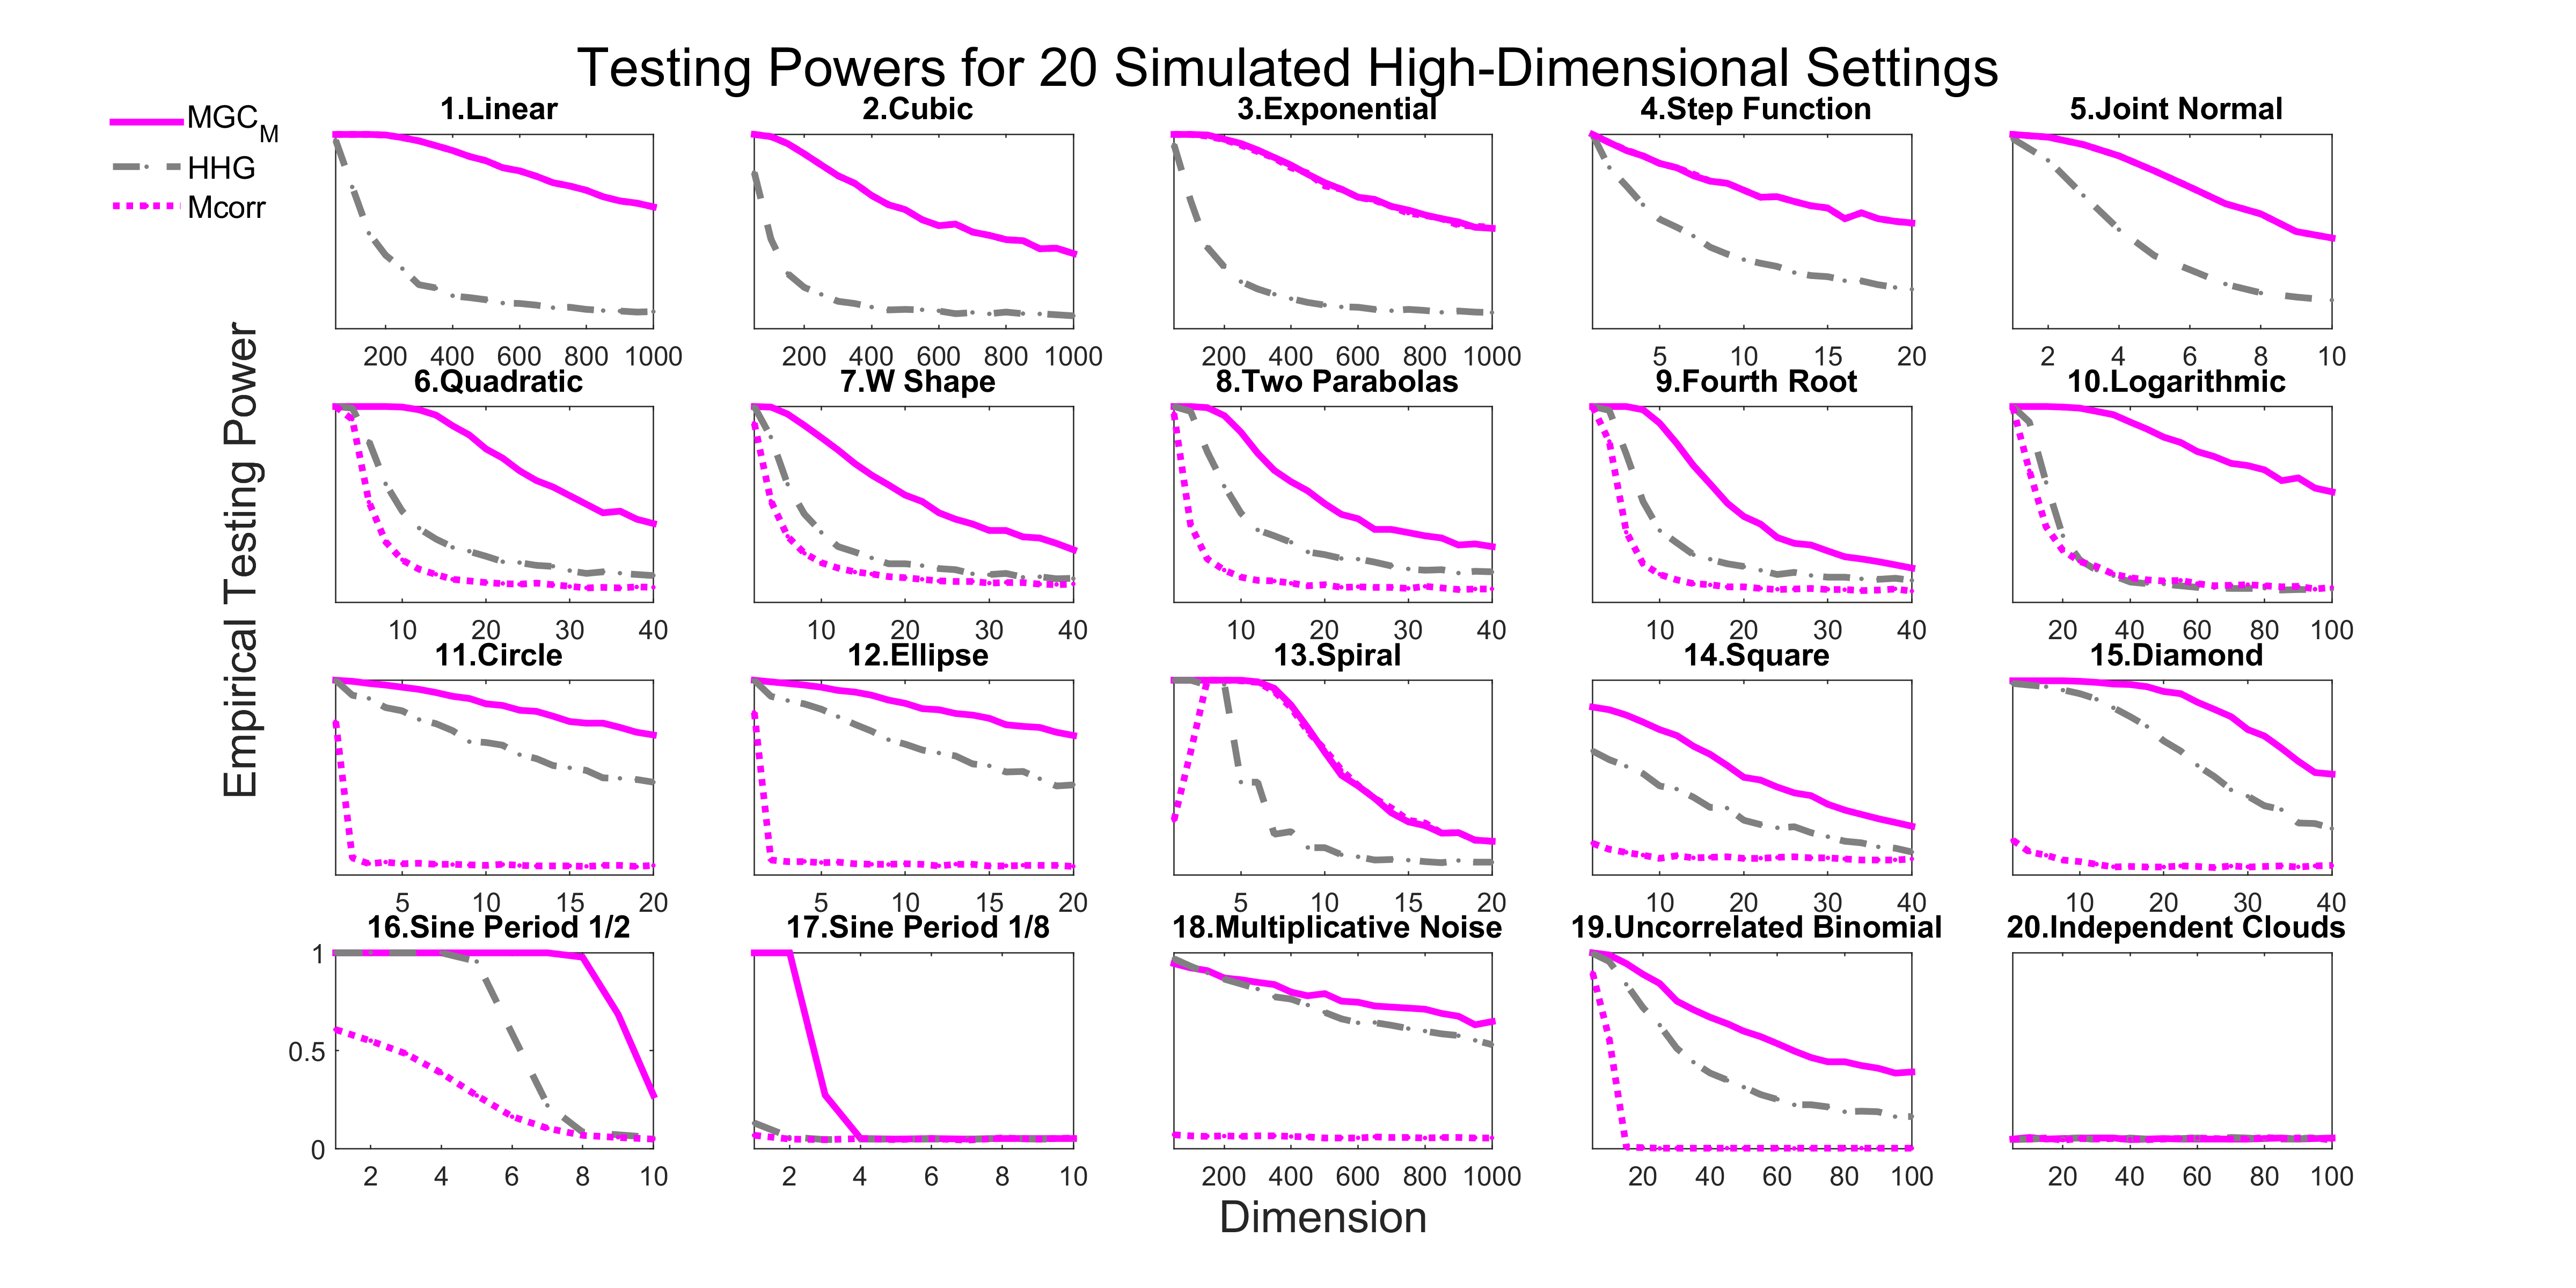
\includegraphics[width=1.0\textwidth,trim={0 0.5cm 4cm 0},clip]{Figures/FigHDPower}
\caption{Power of Oracle \Mgc, sample \Mgc, \Mcorr, and \Hhg~for $20$ different dependence settings, estimated by Monte Carlo independence tests (see Algorithm \ref{alg:power} in Appendix \ref{appen:algorithms} for details).  
Each panel shows the testing power at significance level $\alpha=0.05$
% \jv{should we include `# of' or just leave it off? technically, isn't everything "# of"?}
versus the dimensionality of $\mb{x}$'s, for $n=100$ samples (the dimensionality of $y$ increases for some settings, see Appendix \ref{appen:function} for details). 
Excluding the independent  setting (\#20), for which all methods yield power $0.05$, as they should, \Mgc~empirically achieves similar or better power than both \Mcorr~\cite{SzekelyRizzo2013a}, its global counterpart, and \Hhg~\cite{HellerGorfine2013}, another state-of-the-art method, for almost all settings and all dimensions. 
}
\label{f:nD}
\end{figure}

Figure~\ref{f:nD} shows  the power of each test for all $20$ settings with sample size fixed at $n=100$, but with dimensionality of \mbx~increasing (the dimensionality of \mby~increases in only a subset of the settings; see Appendix \ref{appen:function}).  
%
The advantage of Oracle \Mgc~over \Mcorr~and \Hhg~is stark, with sample \Mgc~performing very close to Oracle \Mgc. For the nearly linear settings, \Mgc~and \Mcorr~are almost identical and significantly better than \Hhg~for all dimensionalities.  For the remaining nonlinear dependencies, \Mgc~achieves power levels that are superior to that of \Hhg~and \Mcorr~for almost all functions, often by a significant margin.  For the independent simulation, all tests yield power at the significance level $\alpha$,  indicating no more false positives than expected.
More exhaustive benchmark experiments, including those focusing on the one-dimensional scenarios,
in which we also compare to \Mantel~and \Dcorr, 
as well as the multiscale variants of both \Mantel~and \Dcorr, 
 are qualitatively similar, and are therefore relegated to Figure~\ref{f:1DAll} and~\ref{f:nDAll}.


\subsection*{\Mgc~Empirically Dominates Global Counterparts}

The above results demonstrate that converting \Mcorr, a global generalized correlation coefficient, to Oracle \Mgc, its multiscale variant, always improves (or does not diminish) the testing power for all considered settings, regardless of the dimensionality and sample size.  This led us to explore whether the multiscale variant of other generalized correlation coefficients would behave similarly.  Specifically, we consider the \Mantel~and \Dcorr~tests, in addition to \Mcorr, and for each, we develop a multiscale variant (see Appendix \ref{appen:methods} for details). 
Figure \ref{f:pp} shows slopegraphs comparing each of the three global correlations with their corresponding Oracle \Mgc~test, as well as global \Mcorr~vs its sample \Mgc.  The top row shows for each of the $20$ settings, with dimensionality of \mbx's and \mby's  fixed at one, the  power averaged over different sample sizes as in Figure~\ref{f:1DAll}.  The bottom row shows the same, but power is averaged over dimensionality of \mbx~while sample size is fixed at $n=100$ as in Figure~\ref{f:nD} and~\ref{f:nDAll}.  In all $40$ settings, for both low and high-dimensions, and for both low and high sample sizes, multiscale methods always either improve on testing power (for nonlinear settings) or keep it almost constant (for linear and independent settings). 

\begin{figure}
  \centering
  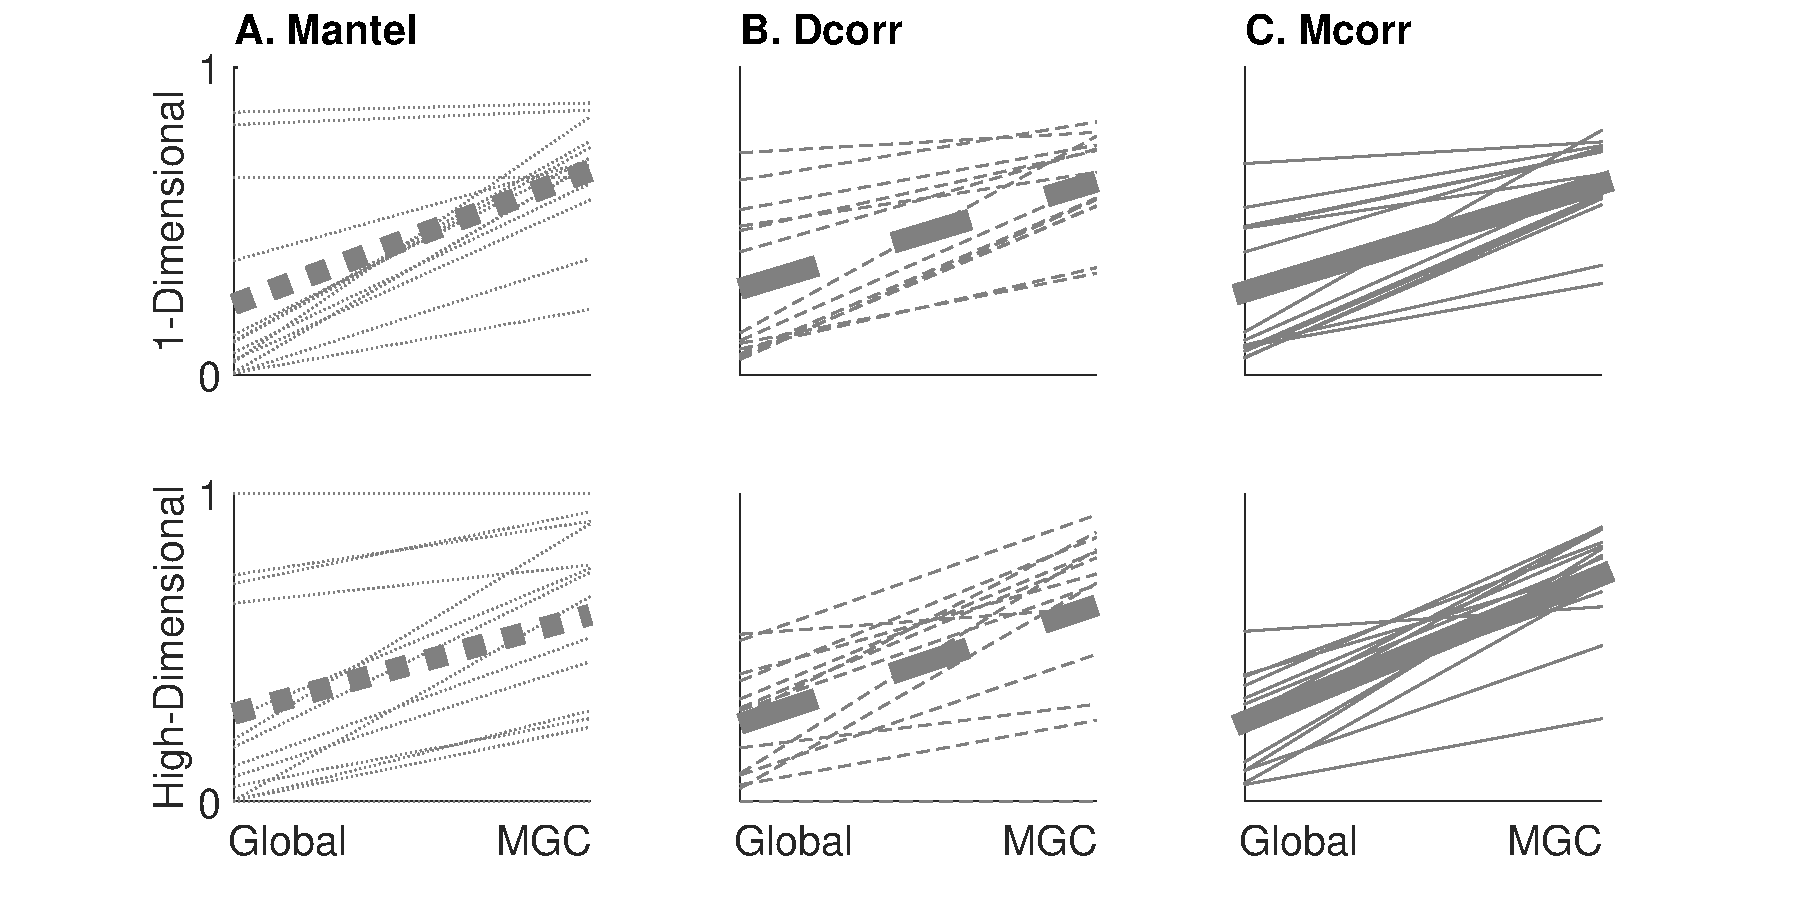
\includegraphics[width=1.0\textwidth,trim={2cm 0 3cm 0},clip]{Figures/FigSlope}
  \caption{
Slopegraphs comparing average power of three different global correlation tests and their respective Oracle \Mgc~(O\Mgc), as well as global \Mcorr~vs its sample \Mgc~(S\Mgc).  Each panel shows average power for settings 6-19, because Oracle \Mgc~equals the global correlation for settings 1-5 and  20. 
The left side of each panel shows the global correlation's average power, and 
the right side shows the corresponding \Mgc's average power. The thick line shows the average within that panel. 
One-dimensional power is averaged over sample size (top)  and high-dimensional power is averaged over dimensionality (bottom), corresponding to Figures~\ref{f:1DAll} and~\ref{f:nDAll}, respectively.
This figure suggests that \Mgc~theoretically dominates its global counterparts, which we prove. 
}
\label{f:pp}
\end{figure}


% 31 lines; target = 64
\subsection*{Discovery of Dependency Across Scales}
\label{main3}

The above sections only demonstrate that \Mgc~provides excellent power, but not that \Mgc~reveals the optimal scales of dependence. 
Figure~\ref{f:powermaps} provides the multiscale power maps for all 20 different high-dimensional scenarios, illustrating how the power of local correlations change with  neighborhood size.
For nearly linear dependencies (1-5), the best neighborhood choice always includes the largest scale, i.e., $k=l=n$. For all strongly nonlinear dependencies (6-19), Oracle \Mgc~chooses smaller scales for $x$ or $y$. Thus a global optimal scale implies a nearly linear dependency, otherwise the dependency is strongly non-linear.
Furthermore, similar dependencies have similar local correlation structure, and thus similar optimal scales. For example, (9) and (10), though very different functions analytically, are qualitatively similar, and yield very similar multiscale power maps.
Similarly,  (16) and (17) are trigonometric functions, and they share a narrow range of significant local correlations.
And both circle (11) and ellipse (12), as well as square (14) and diamond (15), are closely related functions, and have similar multiscale power maps. 
Note that the local structures can be similarly identified by the p-value or test statistic map, and there always exists a large region of local scales that are nearly equally significant in the multiscale maps, which are two important observations that we utilize to design sample \Mgc~in algorithm~\ref{alg:sample_mgc}.


\begin{figure}[htbp]
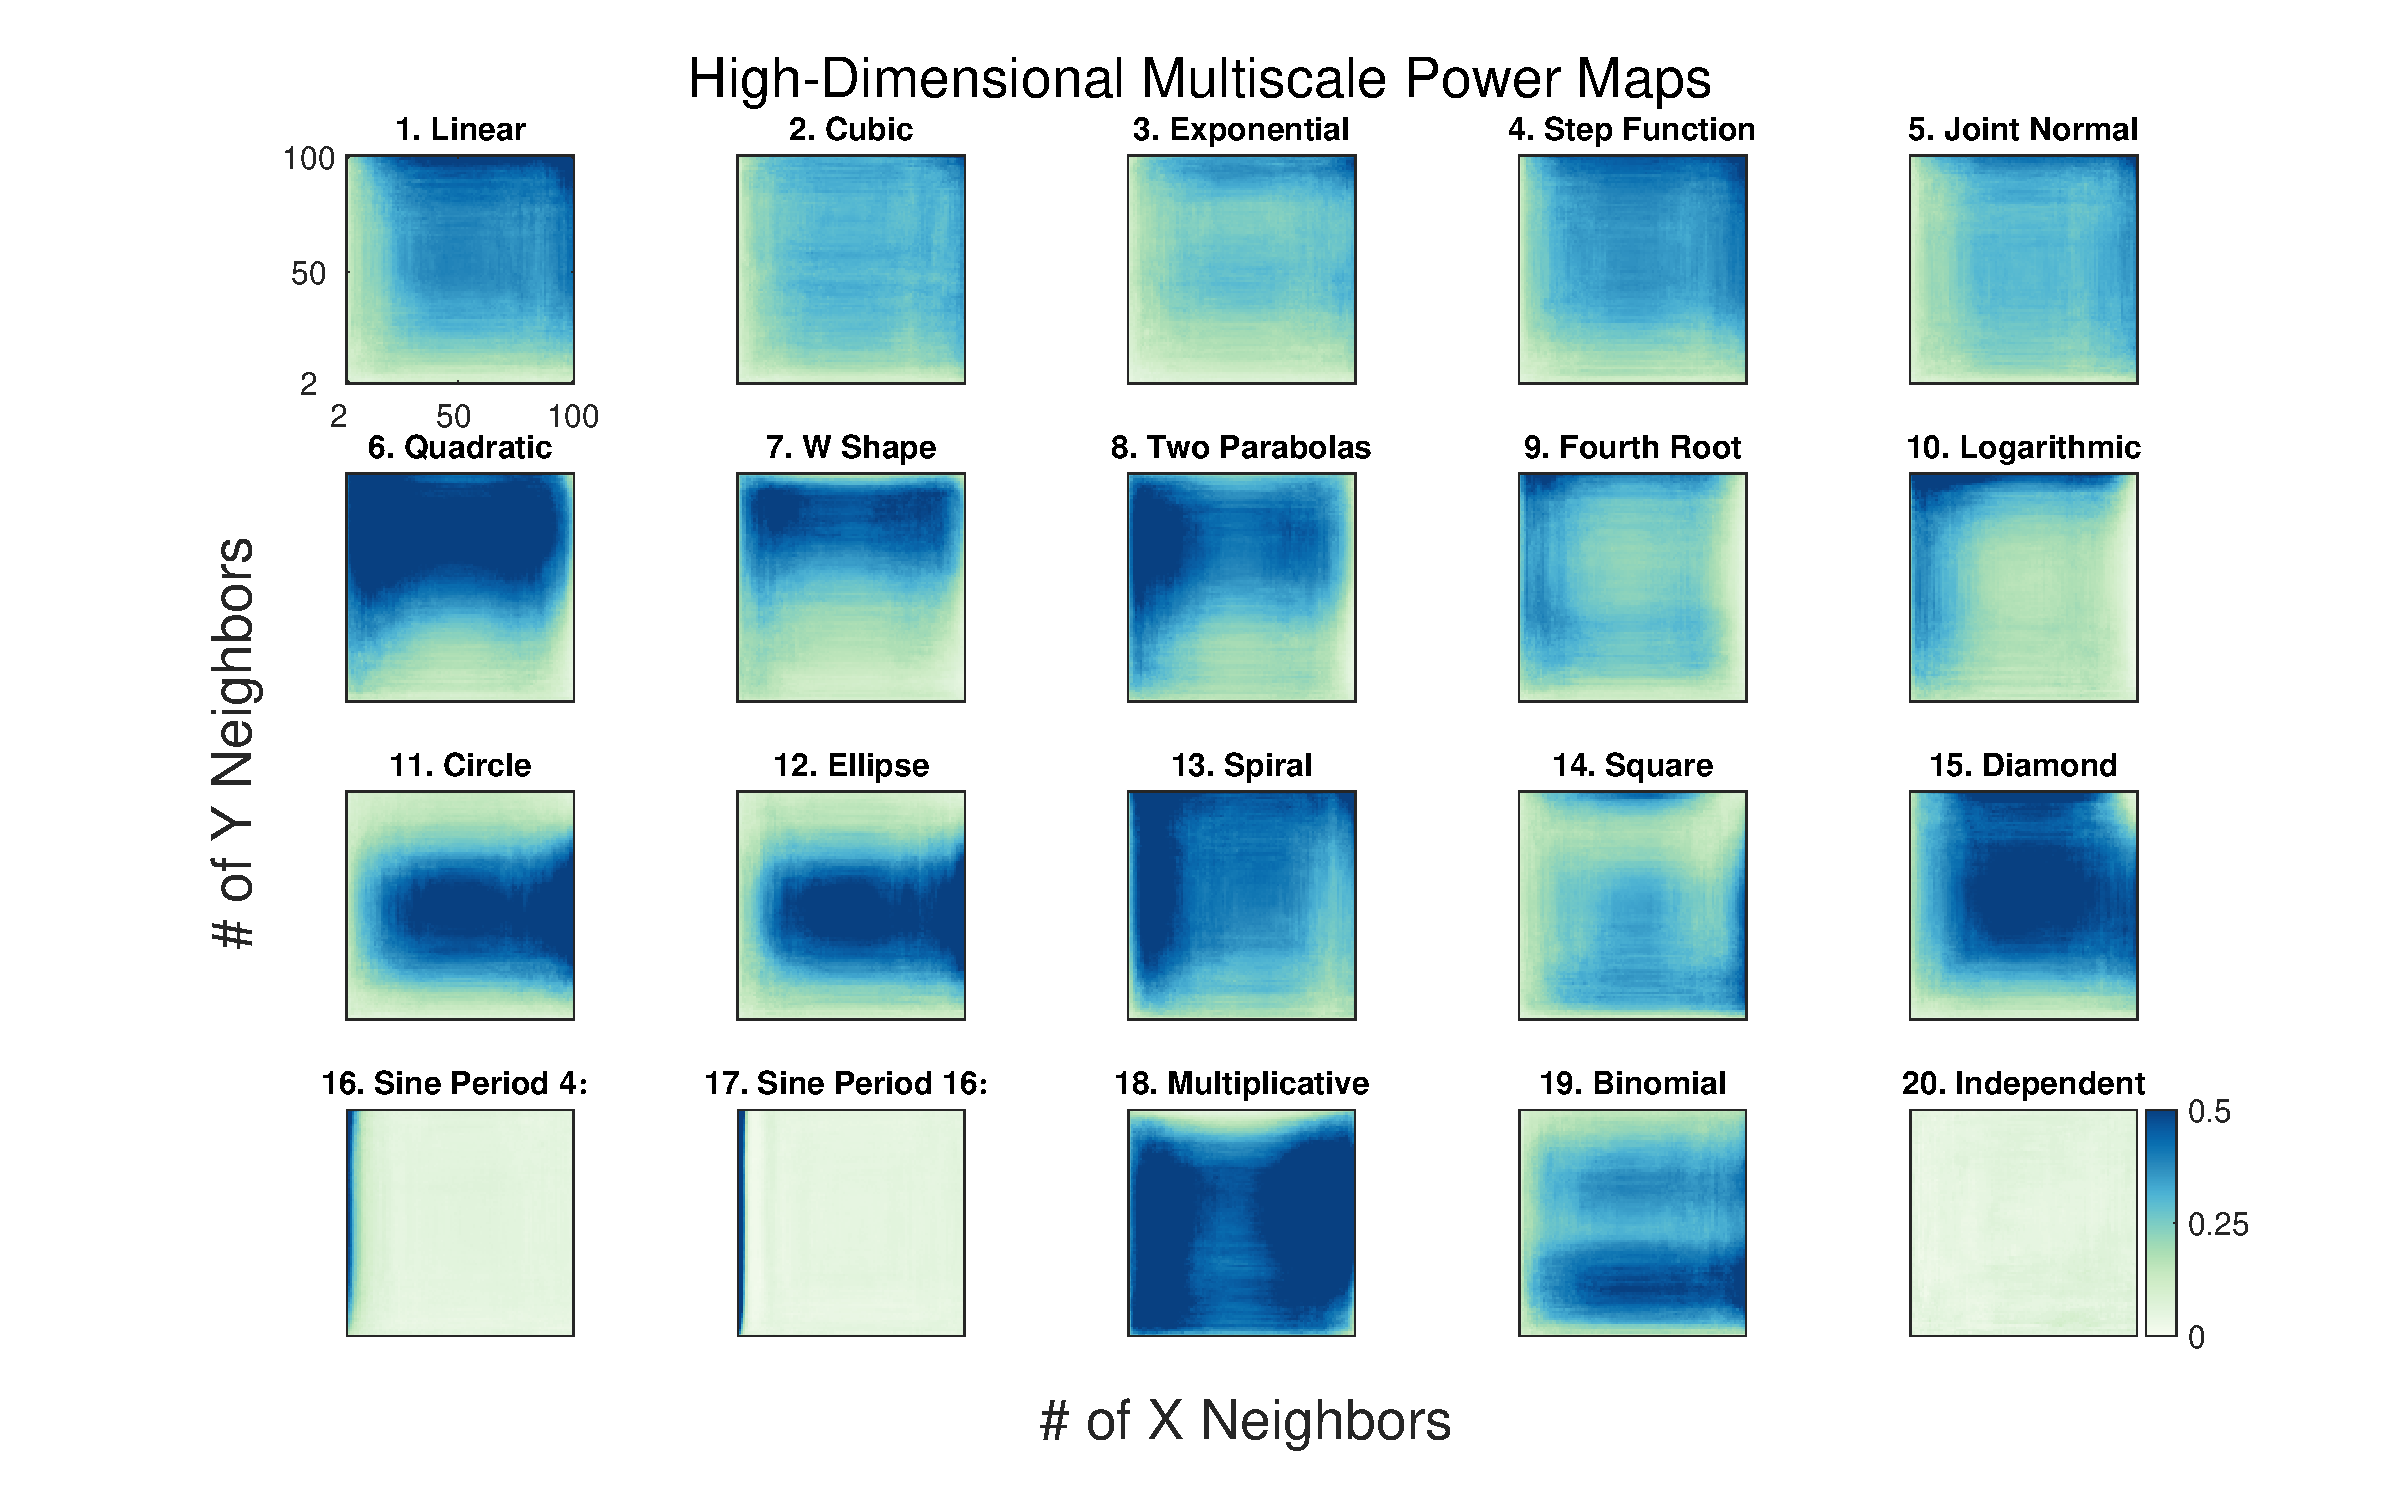
\includegraphics[width=1.0\textwidth,trim={3cm 0.5cm 2.5cm 0.5cm},clip]{Figures/FigHDHeat}
\caption{Multiscale Power Maps reveal the influence of neighborhood size on \Mgc~testing power.
For each of the 20 panels, the abscissa and ordinate denote the number of neighbors for $X$ and  $Y$, respectively. For each simulation, the sample size is $n=100$,  and the dimension is determined by the largest dimension for Oracle \Mgc~to have power exceeding $0.5$ at significance level  $0.05$. Each simulation yields a different multiscale power map, and the global scale is optimal only for nearly linear dependencies, highlighting that \Mgc~not only detects the mere existence of dependency, but also reveals its  structure.}
\label{f:powermaps}
\end{figure}


\subsection*{\Mgc~Theoretically Dominates its Global Counterparts}
\label{s:theory}

To theoretically investigate the performance of \Mgc~requires formalizing the hypotheses. 
Assume $(\mb{x}_i,\mb{y}_i)$ is independently identically distributed as $(\mbx,\mby)$ for $i=1,\ldots,n$. If \mbx~and \mby~are independent, then it  follows that $f_{xy}=f_x f_y$; in other words, for independent data, the joint distribution equals the product of the marginals $f_x$ and $f_y$.  Therefore, we have the following :
\begin{align*}
& H_{0}: f_{xy}=f_{x}f_{y},\\
& H_{A}: f_{xy} \neq f_{x}f_{y}.
\end{align*}
The power of a test is defined as the probability that it correctly rejects the null hypothesis when the null hypothesis is indeed false.
% As defined above, 
A test is consistent if its power converges to one as sample size increases when the null is false, and has power equal to the type $1$ error level when the null is true.
Let $\G_t$ denote a global generalized correlation coefficient based test statistic, that is, $t$ might indicate \Mantel, \Dcorr, or \Mcorr, and let $\beta_n(\G_t^*)$ denote the power of the corresponding Oracle multiscale version for $n$ samples; and we drop the subscript when considering asymptotic power.
Recall from the work of Szekely et al. that \Dcorr~and \Mcorr~are both consistent tests. More specifically, \Dcorr~is consistent whenever $f_{xy}$ has finite dimension and bounded variance, and \Mcorr~is consistent even as dimension increases to infinity.  Denote the set of distributions satisfying consistency for a given test by $\mc{F}_t$, where $t$ indicates which test we are referring to. Then, we have the following theorem:
\begin{thm}
\label{thm1}
$\beta_n(\G_t^*) \rightarrow 1$ as $n \to \infty$ for all $f_{xy}$ in $\mc{F}_t$.
In words, Oracle \Mgc~is consistent against all dependent alternatives for which its global counterpart is consistent. 
\end{thm}


For finite samples, we consider two different kinds of dependencies.
For linear dependencies,  the optimal \Mgc~scale was empirically always the global one (recall Figures~\ref{f:powermaps} and \ref{f:powermaps1}). We therefore conjectured and proved the following:
\begin{thm}
\label{t:linear}
If $\mb{x}$ is linearly dependent on $\mb{y}$, then for any $n$ it always holds that
\begin{equation}
\beta_n(\G_t^*) = \beta_n(\G_t).
\end{equation}
In words, the global scale is the optimal scale for Oracle \Mgc~for linearly dependent data.
\end{thm}

Under nonlinear dependencies and finite sample sizes (which characterizes essentially all real data), we noted that \Mgc~typically achieved better power than its corresponding global correlation. 
We therefore conjectured and proved the following:
\begin{thm}
\label{t:non}
There exists $f_{xy}$ and $n$ such that
\begin{equation}
\beta_n(\G_t^*) \geq \beta_n(\G^{k,l}_{t}) > \beta_n(\G_{t}).
\end{equation}
In words, for finite samples, many different scales of \Mgc~can be better than the global scale under certain nonlinear dependency.
\end{thm}
Note that Theorem~\ref{t:linear} and Theorem~\ref{t:non} hold for any of the \Mgc~varieties, including  \Dcorr, \Mcorr, and \Mantel.
%
The proofs of Theorem~\ref{t:linear} and \ref{t:non} are both in Appendix \ref{appen:proofs}.  The proof of Theorem~\ref{t:linear} is straightforward.  The proof of Theorem~\ref{t:non} is a constructive one. More specifically, we constructed a quadratic function and sampled data a finite number of times and computed the exact p-value for both \Mgc~and \Dcorr, proving that \Mgc~has higher power in this setting. This shows that \Mgc~can outperform its global counterpart even for the most modestly nonlinear functions.  Because any function can be approximated by a polynomial expansion \cite{RudinBook}, the proof of Theorem~\ref{t:non} suggests that \Mgc~is able to outperform its corresponding global correlation on a wide variety of nonlinear functions, which is indeed the case throughout the numerical simulations. 

Taken together, the three theorems above lead to the main theoretical result of this manuscript:
\begin{thm} \label{t:dominate}
Oracle \Mgc~dominates its global counterpart, meaning that \Mgc~is always as good as (in linear settings), and sometimes better than (in nonlinear settings), its corresponding global correlation coefficient, even in finite samples. 
\end{thm}

To our knowledge, this is the first domination theorem in dependence testing, and follows immediately from Theorems \ref{thm1}, \ref{t:linear}, and \ref{t:non}.


\subsection*{Real Data Experiments}
\label{numer3}

\subsubsection*{Brain Activity vs. Personality} 

Our first real data experiment investigates whether there is any dependency between  brain activity and personality.
Adelstein et al. \cite{AdelsteinEtAl2011} were able to detect dependence between certain regions and dimensions of personality, but lacked the tools to test for dependence of the whole brain activity against all five dimensions of personality. 
In this dataset, we have $n=42$ subjects, and for each we obtained  $197$ time-steps of resting-state functional MRI activity, as well as the subject's five-factor personality trait as quantified by  the NEO Personality Inventory-Revised  \cite{Costa1992}. 
The raw brain activity was processed using CPAC \cite{CPAC2015} resulting in $197$ brain regions.
To apply \Mgc, two metrics are required. For the brain activity modality, we ran a spectral analysis on each region, bandpassed and normalized it, and then calculated the Kullback-Leibler divergence across regions to obtain a similarity matrix across all power of regions.  We then used  the normalized Hellinger distance to compute distances between each subject. 
For the five-factor personality data, we  used the Euclidean distance.


Figure \ref{f:real}{\color{magenta}A}  shows that many local scales yield significant p-values ($\approx 0.01$), whereas the global scale fails to detect this significant dependence. In fact, all previously proposed dependence tests under consideration (\Mantel, \Dcorr, \Mcorr, or \Hhg) fail to detect dependence at a significance level of $0.05$, and only \Mgc~provides  insight into the scales of dependence (see Table \ref{t:real}).

\subsubsection*{Brain Shape vs. Disease} 


Our next experiment investigates whether brain shape and disease status are dependent on one another.  Previous investigations have linked major depressive disorder to the hippocampus shape \cite{ParkEtAl2008,PosenerEtAl2003}, though global tests were unable to detect a statistically significant dependence structure at the $\alpha=0.05$ level.
This brain shape versus disease dataset consists of $n=114$ subjects. Each subject has a structural MRI scan as well as a discrete variable indicating whether the subject is clinically depressed $(2)$, high-risk $(1)$, or non-affected $(0)$.  From the MRI data, previous work  extracted both the left and right hippocampi.   For the brain shape modality, they computed the interpoint comparison matrices using a nonlinear landmark matching approach \cite{ParkEtAl2008,BegEtAl2005}. For the  disorder variable, we add white noise bounded by $0.01$ to each label, then form the Euclidean distance (the noise is used to break ties amongst the discrete values and make sure only the diagonal entries of the distance matrix are zero).

Figure \ref{f:real}{\color{magenta}B} provides the p-value map for testing on the right hemisphere using \Mgc. Again, many local scales yield significant p-values, whereas the global scale does not detect a significant dependence  (see Table \ref{t:real}). 

\begin{figure}[htbp]
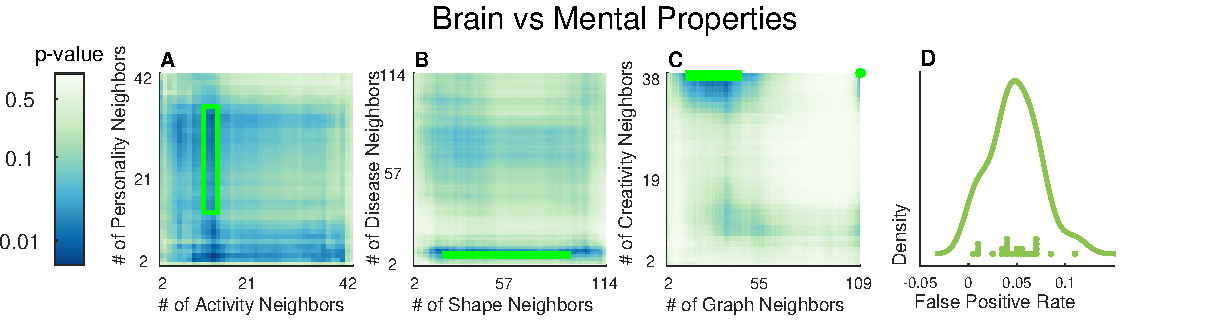
\includegraphics[width=1.0\textwidth,trim={0 0 1.5cm 0},clip]{Figures/FigReal}
\caption{Sample \Mgc~discovers the scales of dependence between various brain and mental properties when they exist, and does not detect dependence when it does not exist.  The left three panels show multiscale p-value maps and their corresponding estimated optimal scales for three different settings: \textbf{A.}  brain activity vs. five-factor personality model, \textbf{B.}  brain shape vs depressive disease, and \textbf{C.} brain networks vs. creativity. Sample size is $42$, $114$, and $109$, respectively, though the ordinate of these panels only goes as high as the largest possible neighborhood size due to repeated entries.  
For all three, \Mgc~yields significant p-value and reveals the optimal scales of dependence (green rectangles).
\textbf{D.} Density estimate for the false positive rates of sample \Mgc~on the brain vs synthetic independent noise experiments, with the actual rate of each experiment shown as dots above the x-axis. The mean $\pm$ standard deviation is $0.0538 \pm 0.0394$ respectively, demonstrating that \Mgc~is a valid test and does not inflate the false positives for these real data.}
\label{f:real}
\end{figure}

\begin{table*}[htbp]
\centering
\begin{tabular}{|c||c|c|c|c|c|}
\hline
Testing Pairs / Methods & Sample \Mgc & \Mantel & \Dcorr & \Mcorr & \Hhg \\
\hline
Activity vs Personality & $\textbf{0.0403}$  & $0.9892$ & $0.6617$ & $0.4441$ & $0.0566$ \\
\hline
Shape vs Disease & $\textbf{0.0276}$  & $0.0772$ & $0.1036$ & $0.1128$ & $0.4581$ \\
\hline
Network vs Creativity & $\textbf{0.0293}$  & $\textbf{0.0100}$ & $\textbf{0.0114}$ & $\textbf{0.0125}$ & $\textbf{0.0316}$ \\
\hline
\end{tabular}
\caption{The p-values for real data testing. \Mgc~is the only method that always finds significant relationship and the only method that ever discovers the underlying optimal scale. Bold indicates significant p-value that is $<0.05$.}
\label{t:real}%
\end{table*}

\subsubsection*{Brain Network vs. Creativity}

The next real data experiment investigates whether brain structural networks are independent of creativity.  Neural correlates of creativity have previously been investigated, though largely using structural MRI and cortical thickness \cite{Jung2009}.  Here, we used data from a previously published result on graph similarity \cite{Koutra15a}. For  $n=109$ subjects, we have both diffusion weighted MRI (dMRI) data as well as the subject's ``creativity composite index'' (CCI).  We processed the raw dMRI data via \Migraine, a pipeline for estimating brain networks from diffusion data \cite{GrayRoncal2013}.   
The brain network metric we used was based on  the semi-parametric test statistic \cite{Tang2016} that tests whether pairs of graphs with labeled vertices are sampled from the same distribution.  This test statistic was developed to reduce  the very high dimensionality of adjacency matrices via employing adjacency spectral graph embedding  \cite{Sussman2013}. For these data, we chose to embed each graph into two dimensions for simplicity. We used Euclidean distance to compare CCI values. 



Figure \ref{f:real}{\color{magenta}C} shows that even a global dependence test can ascertain whether the whole brain network is independent of the subject's creativity.  \Mgc~demonstrates that the signal in this case is largely captured by a global relationship, suggesting that there is relatively little to gain by pursuing nonlinear regression techniques. In this setting with high-dimensional and structured data samples and low-sample size, there is no other obvious way that we could effectively determine that the relationship is approximately linear.



A primary goal of statistical analysis and modeling is to suggest the next experiment or analysis.  For all three of the above investigations, \Mgc~not only found dependence, but also indicated the scales of dependence.  
Thus, to further investigate these datasets --- for example, to build a brain-based assay for any of these mental properties --- we would start by breaking the data into multiple cohorts, whose sizes correspond to the optimal scales detected here.  Without \Mgc, there would be no dependence test-based justification for any subsequent step.
% \jv{sd says: I'm on the fence on whether this should include a hyphen or not. Two hyphens feels excessive ("dependence-test-based"). Thoughts?}


\subsubsection*{Sample \Mgc~Does Not Inflate False Positive Rates} 


In the final experiment, sample \Mgc~is applied to test independence between brain voxel activities and a non-existent stimulus, similar to a pair of studies led by Eklund  \cite{EklundKnutsson2012,Eklund2015}. We considered $25$ resting state fMRI data sets from the 1000 functional connectomes project (\url{http://fcon_1000.projects.nitrc.org/}), consisting of a total of $1$,$583$ subjects.
We used CPAC to estimate regional time-series, in particular, using the sequence of pre-processing decisions determined to optimize discriminability \cite{Wang2016}.  The output for each scan is the resting state fMRI time series data containing $200$ regions of interest for $200$ time-steps.
We then also generate an independent stimulus  by sampling from a standard normal distribution at each time step.  Of course, the brain activity data and the stimuli are independent by construction.
For each brain region, we test: ``Is activity of that  brain region independent of the time-varying stimuli?'' We pool brain activity over all of the samples from the population.
Any regions that are detected significant are false positives by definition.  By testing each brain region separately, we obtain a distribution of false positive rates.  If our test is valid, that distribution should be centered around the significance level, which we set at $0.05$ for this experiment.

To conduct this test, we must construct a distance matrix for brain region activity, and another for the stimulus. For each brain region, $g$, we compute the Euclidean distance pairs of time steps,  $\tilde{a}_{ij}^g=\|\mb{x}_{\cdot i}^g-\mb{x}_{\cdot j}^g\|_2$,  where $\mb{x}_{\cdot i}^g$ denotes the population vector of activity of region $g$ at time-step $i$ for all subjects.
For the one-dimensional stimulus, we similarly compute the Euclidean distance between the stimulus values at each pair of time-steps: $\tilde{b}_{ij}= \|y_i - y_j\|_2$.
Note that the distance matrices at different brain regions are distinct, but the stimulus is the same for all brain regions during the same experiment.


For each data set, the above test is carried out for each brain region; the false positive rates of sample \Mgc~for each dataset are shown in Figure~\ref{f:real}{\color{magenta}D}, which are centered around the critical level $0.05$, as it should be.
In contrast, many standard parametric methods for fMRI analysis, such as generalized linear models, can significantly increase the false positive rates, depending on the data and pre-processing details \cite{EklundKnutsson2012,Eklund2015}. Moreover, even the proposed solutions to those issues make linearity assumptions, thereby limiting detection to only a small subset of possible dependence functions.

\subsection*{Discussion}
\label{conclu}

We propose multiscale generalized correlation (\Mgc) to discover the presence and scales of dependence across disparate properties of data.
We proved that Oracle \Mgc~dominates global approaches in finite samples.  This proof relies on showing first that \Mgc~performs as well as global approaches in certain settings (the linear ones), and then showing that \Mgc~performs \emph{better} than global approaches in other settings (nonlinear ones). 
We further empirically demonstrate via simulations that \Mgc~outperforms global methods regardless of the dimension, sample size, or nonlinearity.  Moreover, in addition to a consistent test, \Mgc~provides a map encoding which scales contain the dependence structure. 
In real data experiments, \Mgc~reveals dependence where global methods fail, discovers the scale of dependence where global methods succeed, and does not falsely detect signals when there are none.


Several other approaches to dependence detection are worth mentioning.
First, a method closely related to distance correlation tests,  is the kernel-based independence test  \cite{GrettonEtAl2005, GrettonGyorfi2010, GrettonEtAl2012}.  Recent work has demonstrated the equivalence between these kernel tests and  energy statistics  \cite{SejdinovicEtAl2013, RamdasEtAl2015}. Thus, we may be able to glean further insights by casting \Mgc~within the kernel framework. Specifically, more efficient tests using asymptotic null distribution approximations for our multiscale tests are possible.
Second, Dumcke et al. \cite{Dumcke2014} recently proposed a related nearest-neighbor based test.  Unfortunately, their proposed test requires estimating relatively high-dimensional densities, and therefore, does not perform particularly well, nor does it have strong theoretical support.
Finally, Reshef et al. \cite{Reshef2011} and Heller et al. \cite{heller2016consistent} are both $1$-dimensional tests, and therefore, not appropriate for our applications (see \cite{SimonTibshirani2012} and \cite{reshef2015empirical} for extensive simulation comparisons demonstrating extensions of their original work).




 \Mgc~can be thought of as a regularized, or sparsified variant of generalized correlation coefficients.  Regularization is central to high-dimensional and ill-posed problems, where dimensionality is larger than sample size.  Thus, it is not surprising that regularizing interpoint comparison matrices yields improved performance.  This connection, however, between dependence testing and regularization is apparently novel.  It opens the door towards considering other regularization techniques for both generalized correlation based dependence testing, and other testing approaches such as \Hhg. In particular, \Hhg~can be thought of as averaging over all scales, rather than regularizing to only consider the optimal ones. The Reshef approach can be thought of similarly.  Therefore, we suspect that this idea could immediately impact other statistical testing frameworks.



There are a number of additional potential extensions of this work.  First, theoretical guidance for choosing the optimal scale for finite samples  in the absence of training data, would be desirable. 
In this work we proved that there exist local scales that improve upon the global scale, and demonstrated that sample \Mgc~yields tests with power very close to the optimal power, often better than \Hhg~and \Mcorr, and with significant p-values and accurate optimal scale estimation for the real data.  But more theory connecting Oracle \Mgc~and  Sample \Mgc~will yield further insight.


Second, \Mgc~requires a pair of metrics, one for each data type. In this work we selected such metrics using domain knowledge, and mitigated the potential inopportune choice of metric via locality tuning.  If we were able to choose the optimal metric for a given dataset, this would possibly obviate the need for locality, and further improve power. Szekely et al. investigated different norms and exponents to ascertain the impact of different metrics, but was unable to determine optimality.
Metric learning \cite{xing2003distance} addresses learning metrics for different exploitation tasks, so perhaps ideas from that literature can be brought to bear on this problems.  Specifically, perhaps a different one-dimensional family of metrics could yield additional insights into choosing an optimal metric and scale.

Third, essentially all of the tests described in this manuscript are quadratic in sample size.  When sample size gets very large, such a computational burden is intractable.  Recent work from Huo and Szekely  has demonstrated efficient algorithms that are linear in sample size  for one-dimensional data \cite{Huo2016}.  Although it is not clear how to extend the Huo and Szekely approach  to multidimensional data, a subsampling strategy seems viable.  In fact, the multiscale power maps are accurate even when subsampling the data points significantly (not shown), suggesting that subsampling data or pairwise comparisons  could yield an approximate linear time algorithm.  One could also implement \Mgc~using a semi-external computing model \cite{Zheng2016},  which could enable using solid state disk space in a streaming fashion to both speed up computations for big data and enable storing interpoint pairwise comparison matrices larger than what can fit in RAM.

Finally, the notion of multiscale generalized correlations could be used in a wide variety of related exploitation tasks.  In particular, ``energy statistics''---for which $\Dcorr$ and $\Mcorr$ are special cases---have been applied to many different testing scenarios, including goodness-of-fit  \cite{Szekely2005}, analysis of variance  \cite{Rizzo2010}, conditional dependence  \cite{Szekely2014,Wang2015},   and feature selection \cite{LiZhongZhu2012,Zhong2015}.     
\Mgc~is fact can be thought of as implementing two-sample (or even $K$-sample) tests \cite{Szekely2004}, whenever $x$ or $y$ is categorical.  
Thus, further investigation comparing the advances of \Mgc~to standard methods for two-sample tests is appealing.
Testing independence between graphs and node attributes \cite{Fosdick2015} is another immediate potential application.  And while not previously addressed, using the \Mgc~intuition for dimensionality reduction, classification, and regression seem like very promising future directions, especially because \Mgc~reveals the scales of dependence which can easily be employed in such problems.

To facilitate the reproducability of this work, as well as myriad applications and extensions, all source code for performing the experiments, generating figures, and the functions themselves are provided in the website, \website, including both R and MATLAB implementations.


\clearpage
\pagestyle{plain}
\bibliographystyle{Science}
\bibliography{MGCbib}


\section*{Acknowledgment}
% \addcontentsline{toc}{section}{Acknowledgment}
This work was partially supported by the
%
National Security Science and Engineering Faculty Fellowship (NSSEFF),
%
the Johns Hopkins University Human Language Technology Center of Excellence (JHU HLT COE),  the
%
Defense Advanced Research Projects Agency's (DARPA) SIMPLEX program through SPAWAR contract N66001-15-C-4041,
%
the XDATA program of DARPA administered through Air Force Research Laboratory contract FA8750-12-2-0303,
%
the Office of Naval Research contract N00014-12-1-0601,
%
the Air Force Office of Scientific Research contract FA955014-1-0033. The authors thank Dr. Brett Mensh of Optimize Science for acting as our intellectual consigliere, and Dr. Ruth Heller for insightful suggestions regarding sample \Mgc.

\clearpage
\appendix
\setcounter{figure}{0}
\renewcommand\thefigure{A\arabic{figure}}

\section{Simulation Functions}
\label{appen:function}

This section provides the $20$ different dependency functions used in the simulations.  We used essentially the exact same settings as previous publications to ensure a fair comparison \cite{SzekelyRizzoBakirov2007, SimonTibshirani2012, SimonTibshirani2012, GorfineHellerHeller2012}.  We only made changes to add white noise, and a weight vector for higher dimensions, thereby making them more difficult, to better compare all methods throughout different dimensions and sample sizes. We also included a few additional settings.

For each sample $\mb{x} \in \Real^{D}$, we denote $\mb{x}_{[d]}, d=1,\ldots,D$ as the $d^{th}$ dimension of the vector \mbx. For the purpose of high-dimensional simulations, $w \in \Real^{D}$ is a decaying vector with $w_{[d]}=1/d$ for each $d$, such that $w\T \mb{x}$ is a 
% one-dimensional 
weighted summation of all dimensions of \mbx. %, which equals \mb{x}~if $D=1$.
Furthermore, $\mc{U}(a,b)$ denotes the uniform distribution on the interval $(a,b)$, $\mc{B}(p)$ denotes the Bernoulli distribution with probability $p$, $\mc{N}(\mu,{\Sigma})$ denotes the normal distribution with mean ${\mu}$ and covariance ${\Sigma}$, 
$u$ and $v$ represent realizations from some auxiliary random variables, $c$ is a scalar constant to control the noise level (which equals $1$ for one-dimensional simulations and $0$ otherwise), and $\epsilon$ is sampled from an independent standard normal distribution unless mentioned otherwise.

For all of the below equations, $(\mb{x},\mb{y}) \overset{iid}{\sim} f_{xy} = f_{y|x} f_x$. For each setting, we provide the space of $(\mb{x},\mb{y})$, and define $f_{y|x}$ and $f_x$, as well as any additional auxiliary distributions.

\setcounter{equation}{0}
\begin{compactenum}
\item Linear $(\mb{x},\mb{y}) \in \Real^{D} \times \Real$,
\begin{align*}
\mb{x} &\sim \mc{U}(-1,1)^{D},\\
\mb{y} &=w\T \mb{x}+c\epsilon.
\end{align*}
\item Cubic $(\mb{x},\mb{y}) \in \Real^{D} \times \Real$:
\begin{align*}
\mb{x} &\sim \mc{U}(-1,1)^{D}, \\
\mb{y} &=128(w\T \mb{x}-\tfrac{1}{3})^3+48(w\T \mb{x}-\tfrac{1}{3})^2-12(w\T \mb{x}-\tfrac{1}{3})+80c\epsilon.
\end{align*}
\item Exponential $(\mb{x},\mb{y}) \in \Real^{D} \times \Real$:
\begin{align*}
\mb{x} &\sim \mc{U}(0,3)^{D}, \\
\mb{y} &=exp(w\T \mb{x})+10c\epsilon.
\end{align*}
\item Step Function $(\mb{x},\mb{y}) \in \Real^{D} \times \Real$:
\begin{align*}
\mb{x} &\sim \mc{U}(-1,1)^{D},\\
\mb{y} &=\mb{I}(w\T \mb{x}>0)+\epsilon,
\end{align*}
where $\mb{I}$ is the indicator function, that is $\mb{I}(z)$ is unity whenever $z$ true, and zero otherwise.
\item Joint normal $(\mb{x},\mb{y}) \in \Real^{D} \times \Real^{D}$: Let $\rho=1/2D$, $I_{D}$ be the identity matrix of size $D \times D$, $J_{D}$ be the matrix of ones of size $D \times D$, and $\Sigma = \begin{bmatrix} I_{D}&\rho J_{D}\\ \rho J_{D}& (1+0.5c) I_{D} \end{bmatrix}$. Then let $\epsilon \sim \mc{N}(0, I_{D})$,
\begin{align*}
(\mb{x}, \mb{y}) &\sim \mc{N}(0, \Sigma). 
% \\\mb{y} &=\mb{y}+0.5c\epsilon.
\end{align*}
\item Quadratic $(\mb{x},\mb{y}) \in \Real^{D} \times \Real$:
\begin{align*}
\mb{x} &\sim \mc{U}(-1,1)^{D},\\
\mb{y}&=(w\T \mb{x})^2+0.5c\epsilon.
\end{align*}
\item W Shape $(\mb{x},\mb{y}) \in \Real^{D} \times \Real$:  $u \sim \mc{U}(-1,1)^{D}$,
\begin{align*}
\mb{x} &\sim \mc{U}(-1,1)^{D},\\
\mb{y}&=4\left[ \left( (w\T \mb{x})^2 - \tfrac{1}{2} \right)^2 + w\T u/500 \right]+0.5c\epsilon.
\end{align*}
\item Two Parabolas $(\mb{x},\mb{y}) \in \Real^{D} \times \Real$: $\epsilon \sim \mc{U}(0,1)$, $u \sim \mc{B}(0.5)$,
\begin{align*}
\mb{x} &\sim \mc{U}(-1,1)^{D},\\
\mb{y}&=\left( (w\T \mb{x})^2  + 2c\epsilon\right) \cdot (u-\tfrac{1}{2}).
\end{align*}
\item Fourth Root $(\mb{x},\mb{y}) \in \Real^{D} \times \Real$:
\begin{align*}
\mb{x} &\sim \mc{U}(-1,1)^{D},\\
\mb{y}&=|w\T \mb{x}|^\frac{1}{4}+\frac{c}{4}\epsilon.
\end{align*}
\item Logarithmic $(\mb{x},\mb{y}) \in \Real^{D} \times \Real^{D}$: $\epsilon \sim \mc{N}(0, I_{D})$
\begin{align*}
\mb{x} &\sim \mc{N}(0, I_{D}),\\
\mb{y}_{[d]}&=2\log_{2}(\mb{x}_{[d]})+3c\epsilon_{[d]},
\end{align*}
for $d=1,\ldots,D$.
\item Circle $(\mb{x},\mb{y}) \in \Real^{D} \times \Real$: $u \sim \mc{U}(-1,1)^{D}$, $\epsilon \sim \mc{N}(0, I_{D})$, $r=1$,
\begin{align*}
\mb{x}_{[d]}&=r \left(\sin(\pi u_{[d+1]})  \prod_{j=1}^{d} \cos(\pi u_{[j]})+0.4 \epsilon_{[d]}\right) \mbox{ for $d=1,\ldots,D-1$},\\
\mb{x}_{[D]}&=r \left(\prod_{j=1}^{D} \cos(\pi u_{[j]})+0.4 \epsilon_{[D]}\right),\\
\mb{y}&= \sin(\pi u_{[1]}).
\end{align*}
\item Ellipse $(\mb{x},\mb{y}) \in \Real^{D} \times \Real$: Same as above except $r=5$.

\item Spiral $(\mb{x},\mb{y}) \in \Real^{D} \times \Real$: $u \sim \mc{U}(0,5)$, $\epsilon \sim \mc{N}(0, 1)$,
\begin{align*}
\mb{x}_{[d]}&=u \sin(\pi u)  \cos^{d}(\pi u) \mbox{ for $d=1,\ldots,D-1$},\\
\mb{x}_{[D]}&=u \cos^{D}(\pi u),\\
\mb{y}&= u \sin(\pi u) +0.4 (D-1)\epsilon.
\end{align*}

\item Square $(\mb{x},\mb{y}) \in \Real^{D} \times \Real^{D}$: Let $u \sim \mc{U}(-1,1)$, $v \sim \mc{U}(-1,1)$, $\epsilon \sim \mc{N}(0,1)^{D}$, $\theta=-\frac{\pi}{8}$. Then
\begin{align*}
\mb{x}_{[d]}&=u \cos\theta + v \sin\theta + 0.05 D\epsilon_{[d]},\\
\mb{y}_{[d]}&=-u \sin\theta + v \cos\theta,
\end{align*}
for $d=1,\ldots,D$.
\item Diamond $(\mb{x},\mb{y}) \in \Real^{D} \times \Real^{D}$: Same as above except $\theta=-\frac{\pi}{4}$.
\item Sine Period $4\pi$ $(\mb{x},\mb{y}) \in \Real^{D} \times \Real$: $u \sim \mc{U}(-1,1)$, $v \sim \mc{N}(0,1)^{D}$, $\theta=4\pi$,
\begin{align*}
\mb{x}_{[d]}&=u+0.02 D v_{[d]} \mbox{ for $d=1,\ldots,D$}, \\
\mb{y}&=\sin ( \theta x )+c\epsilon.
\end{align*}
\item Sine Period $16\pi$ $(\mb{x},\mb{y}) \in \Real^{D} \times \Real$: Same as above except $\theta=16\pi$ and the noise on $\mb{y}$ is changed to $0.5c\epsilon$.
\item Multiplicative Noise $(\mb{x},\mb{y}) \in \Real^{D} \times \Real^{D}$: $u \sim \mc{N}(0, I_{D})$, %$\epsilon \sim \mc{N}(0, I_{D})$,
\begin{align*}
\mb{x} &\sim \mc{N}(0, I_{D}),\\
\mb{y}_{[d]}&=u_{[d]}\mb{x}_{[d]},%+0.5c\epsilon,
\end{align*}
for $d=1,\ldots,D$.
\item Uncorrelated Bernoulli $(\mb{x},\mb{y}) \in \Real^{D} \times \Real$: $u \sim \mc{B}(0.5)$, $\epsilon_{1} \sim \mc{N}(0, I_{D})$, $\epsilon_{2} \sim \mc{N}(0, 1)$,
\begin{align*}
\mb{x} &\sim \mc{B}(0.5)^{D}+0.5\epsilon_{1},\\
\mb{y}&=(2u-1)w\T \mb{x}+0.5\epsilon_{2}.
\end{align*}
\item Independent Clouds $(\mb{x},\mb{y}) \in \Real^{D} \times \Real^{D}$: Let $u \sim \mc{N}(0,I_{D})$, $v \sim \mc{N}(0,I_{D})$, $u' \sim \mc{B}(0.5)^{D}$, $v' \sim \mc{B}(0.5)^{D}$. Then
\begin{align*}
\mb{x}&=u/3+2u'-1,\\
\mb{y}&=v/3+2v'-1.
\end{align*}
\end{compactenum}

For each distribution, $\mb{x}$ and $\mb{y}$ are dependent except  (20); for some settings (11-15) they are conditionally independent upon conditioning on the respective auxiliary variables, while for others they are
 ``directly'' dependent. 
 Given $(\mb{x}_{i},\mb{y}_{i})$ pairs for $i=1,\ldots,n$, set $X=\{\mb{x}_{1},\cdots, \mb{x}_{n}\} \in \Real^{D \times n}$ and $Y=\{\mb{y}_{1},\cdots, \mb{y}_{n}\} \in \Real^{D_y \times n}$, where $D_y$ is the dimensionality of \mby. A visualization of each dependency with $D=D_y=1$ is shown in Figure~\ref{f:dependencies}.


For the increasing dimension simulation in the main paper, we always set $c=0$ and $n=100$, with $D$ increasing.  For types  $5,10,14,15,18,20$, we let $D_y=D$; otherwise, we let $D_y=1$. 
The decaying vector $w$ is utilized for $D>1$ to make the high-dimensional settings more difficult (otherwise, additional dimensions only add more signal).


\section{Supplementary Figures}
\label{appen:figs}





\begin{figure}[htbp]
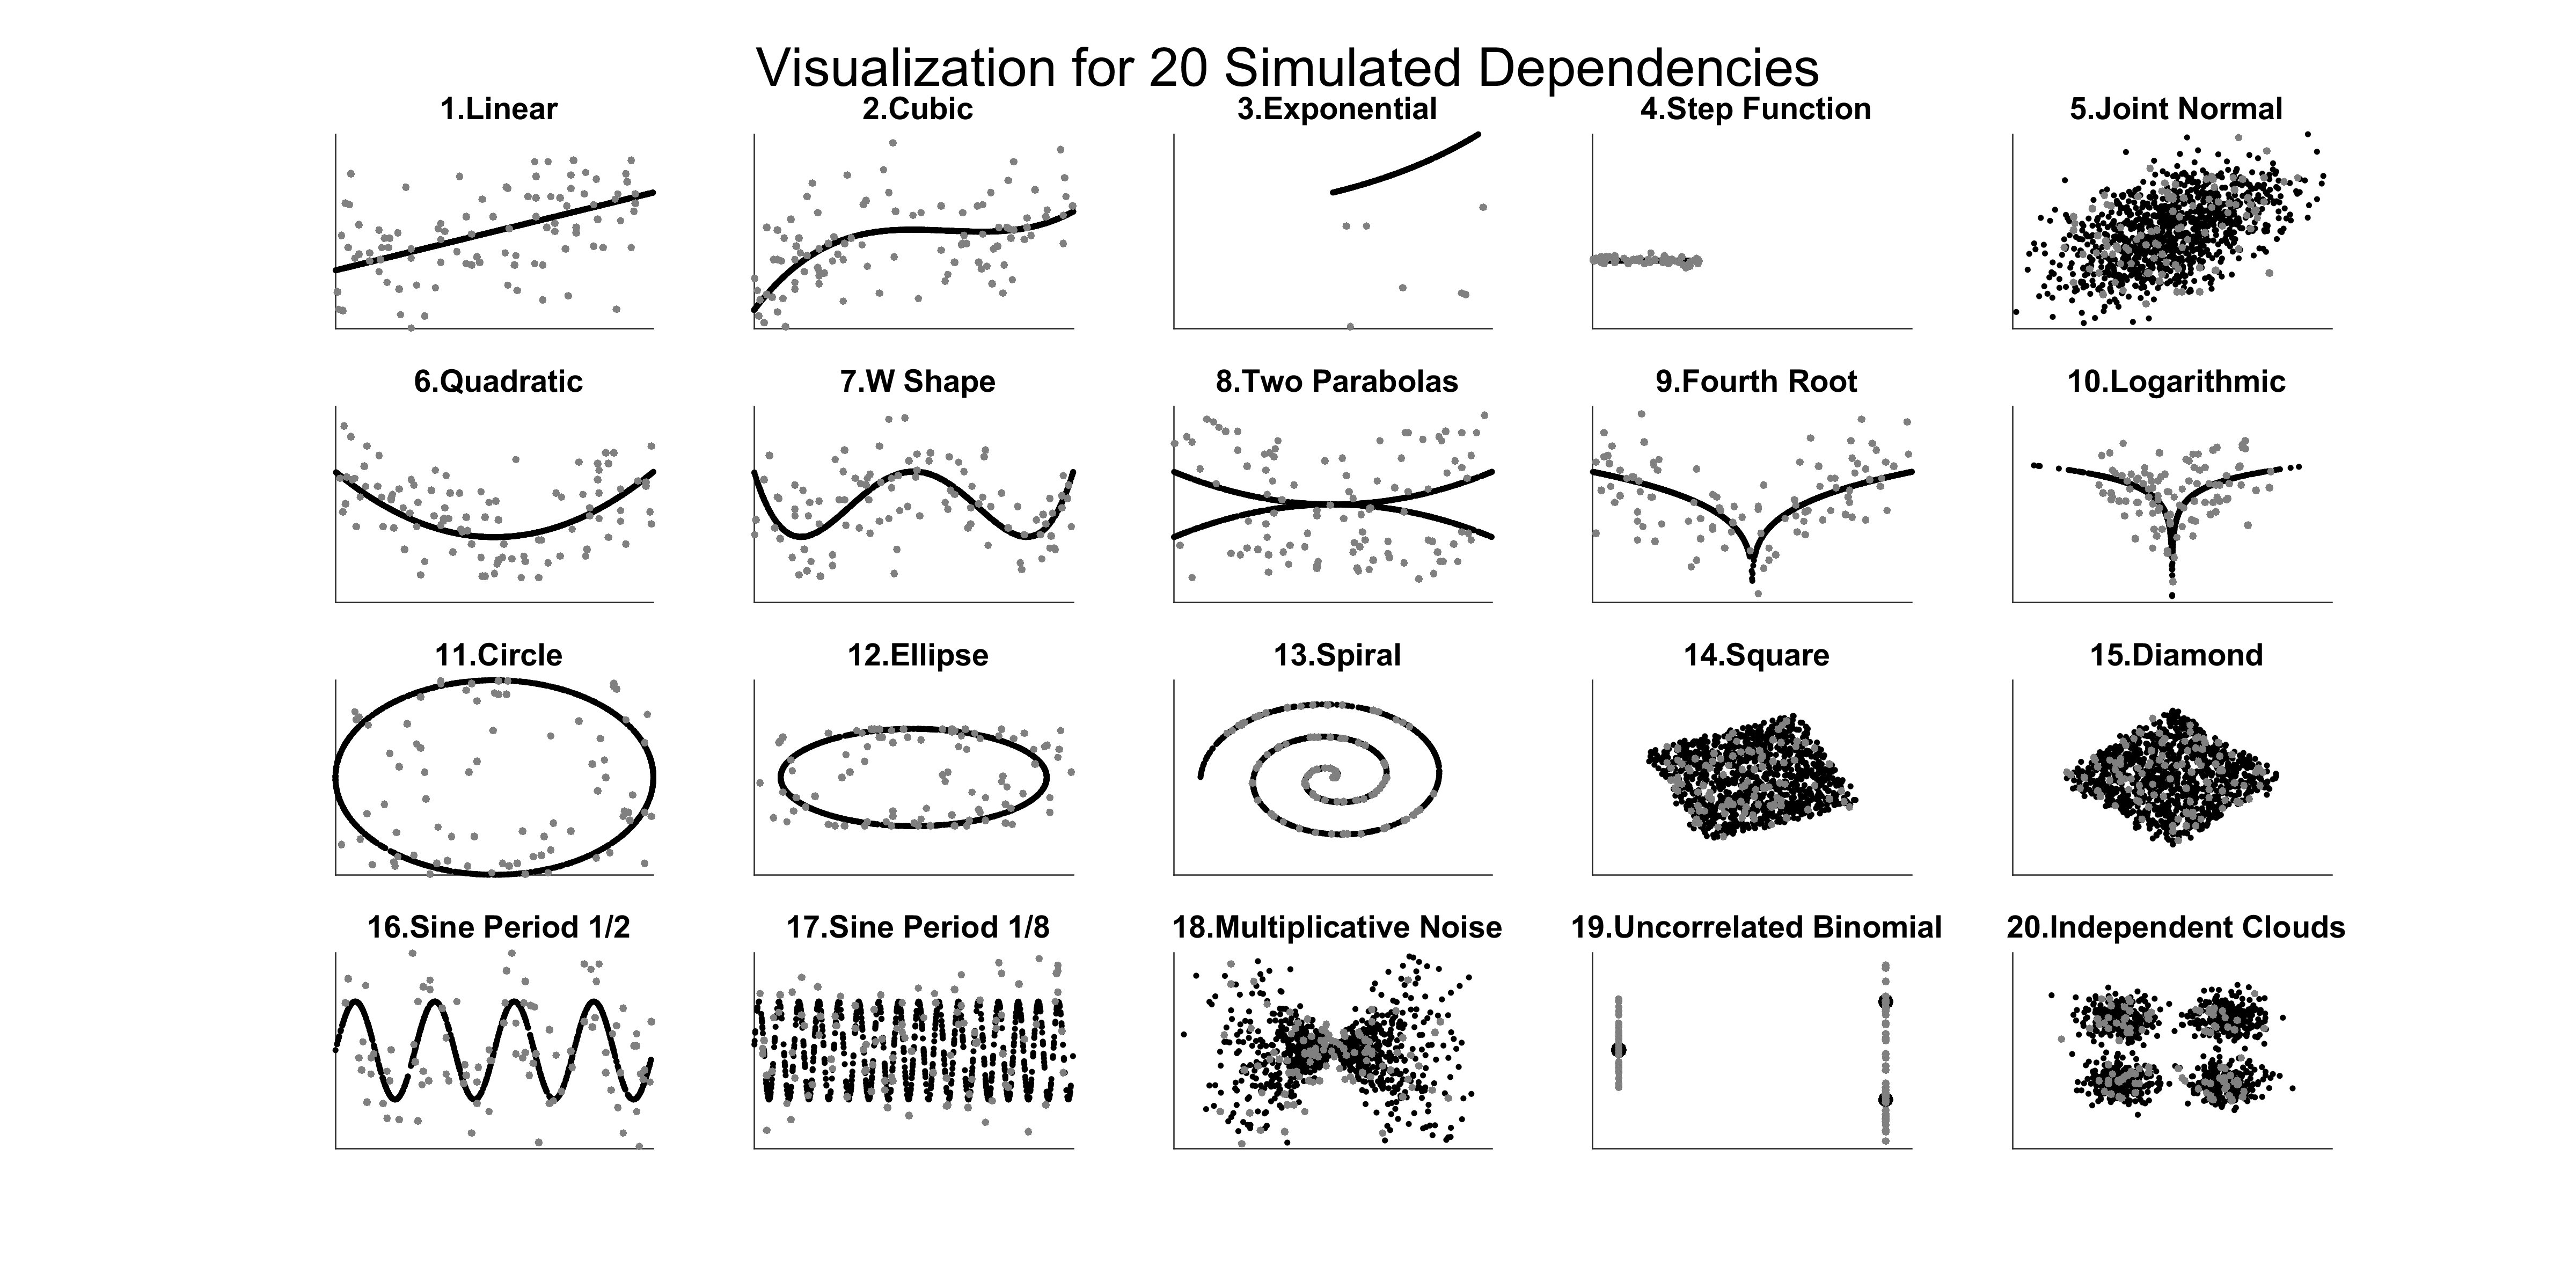
\includegraphics[trim={5cm 1.5cm 4cm 0.5cm},clip, width=1.0\textwidth]{Figures/FigSimVisual}
\caption{Visualization of the $20$ dependencies at $D=D_{y}=1$. For each, we sampled $n=100$ points with noise ($c=1$) to show the actual sample data used for 1-dimensional settings (gray dots). For comparison purposes, we also sampled $n=1000$ points without noise ($c=0$) to highlight each underlying dependency (black dots).
}
\label{f:dependencies}
\end{figure}

\begin{figure}[htbp]
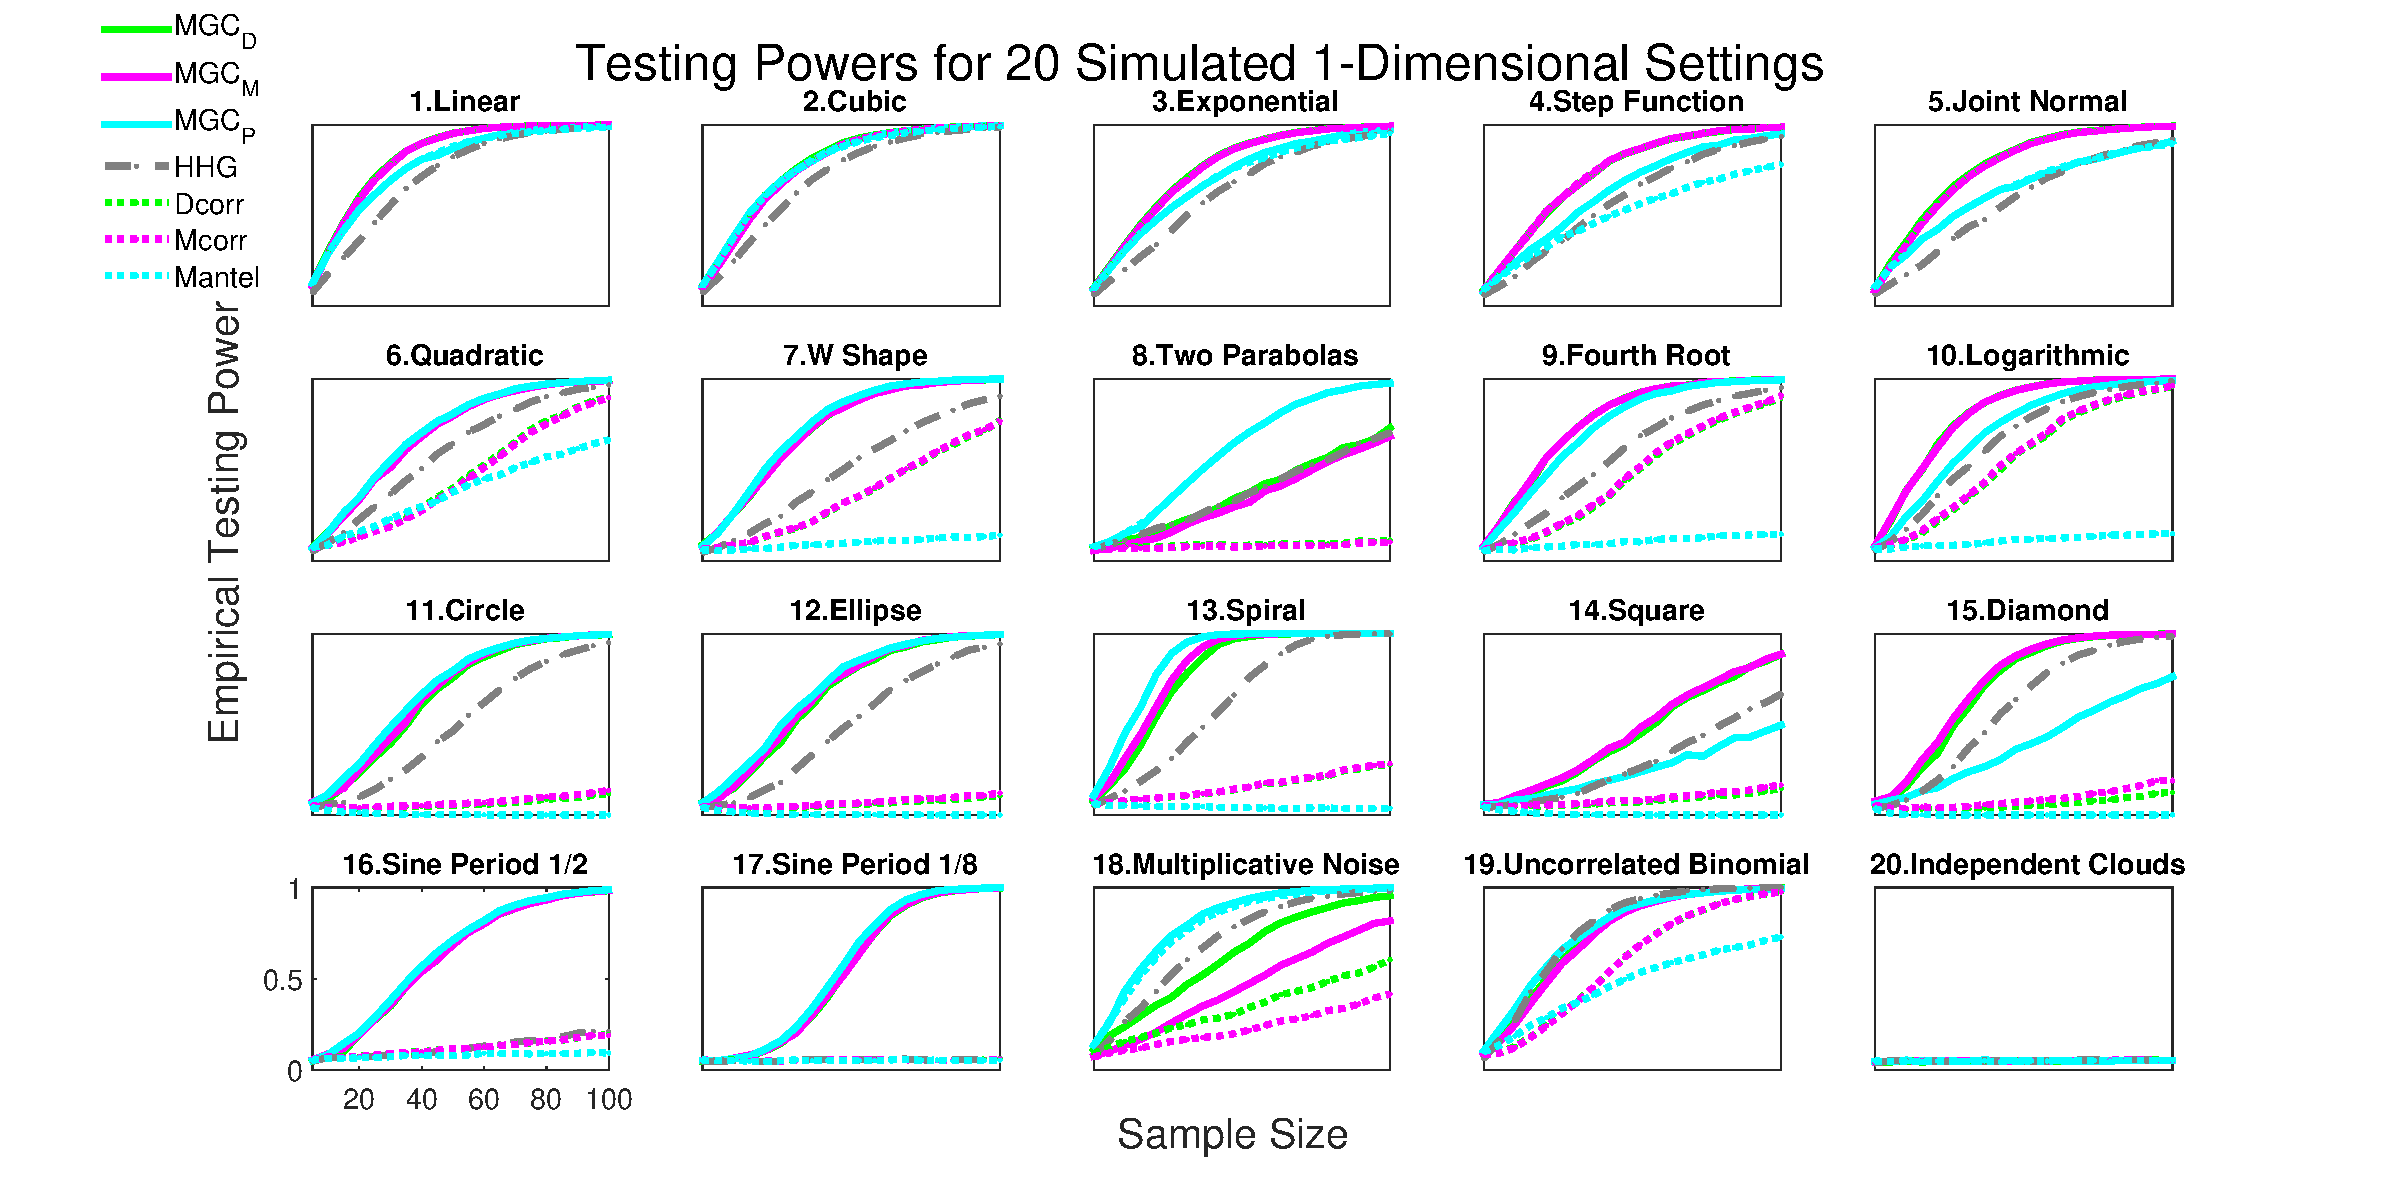
\includegraphics[width=1.0\textwidth,trim={0 0.5cm 4cm 0},clip]{Figures/Fig1DPowerAll}
\caption{
Power of different methods for $20$ different one-dimensional dependence structures, estimated by the empirical distributions of the test statistics under the null and the alternative hypotheses.
 % on the basis of $10$,$000$ Monte-Carlo replicates. $2$,$000$ additional MC replicates are used for optimal scale estimation for \Mgc.
This figure includes seven different tests: \Mantel, \Dcorr, and \Mcorr  (magenta dotted, dashed, and solid lines, respectively), their corresponding \Mgc~counterparts, \Mgcp, \Mgcd, \Mgcm~(green with same line styles), as well as sample \Mgc~(cyan) and \Hhg (gray).
Each panel shows the testing power on the abscissa at a significance level $\alpha=0.05$, and sample size on the ordinate.
Oracle \Mgc~empirically achieves similar or better power than the previous state of the art approaches for all sample sizes on almost all problems, with sample \Mgc~being very close to Oracle \Mgc~and overall superior to other benchmarks.}
\label{f:1DAll}
\end{figure}

\begin{figure}[htbp]
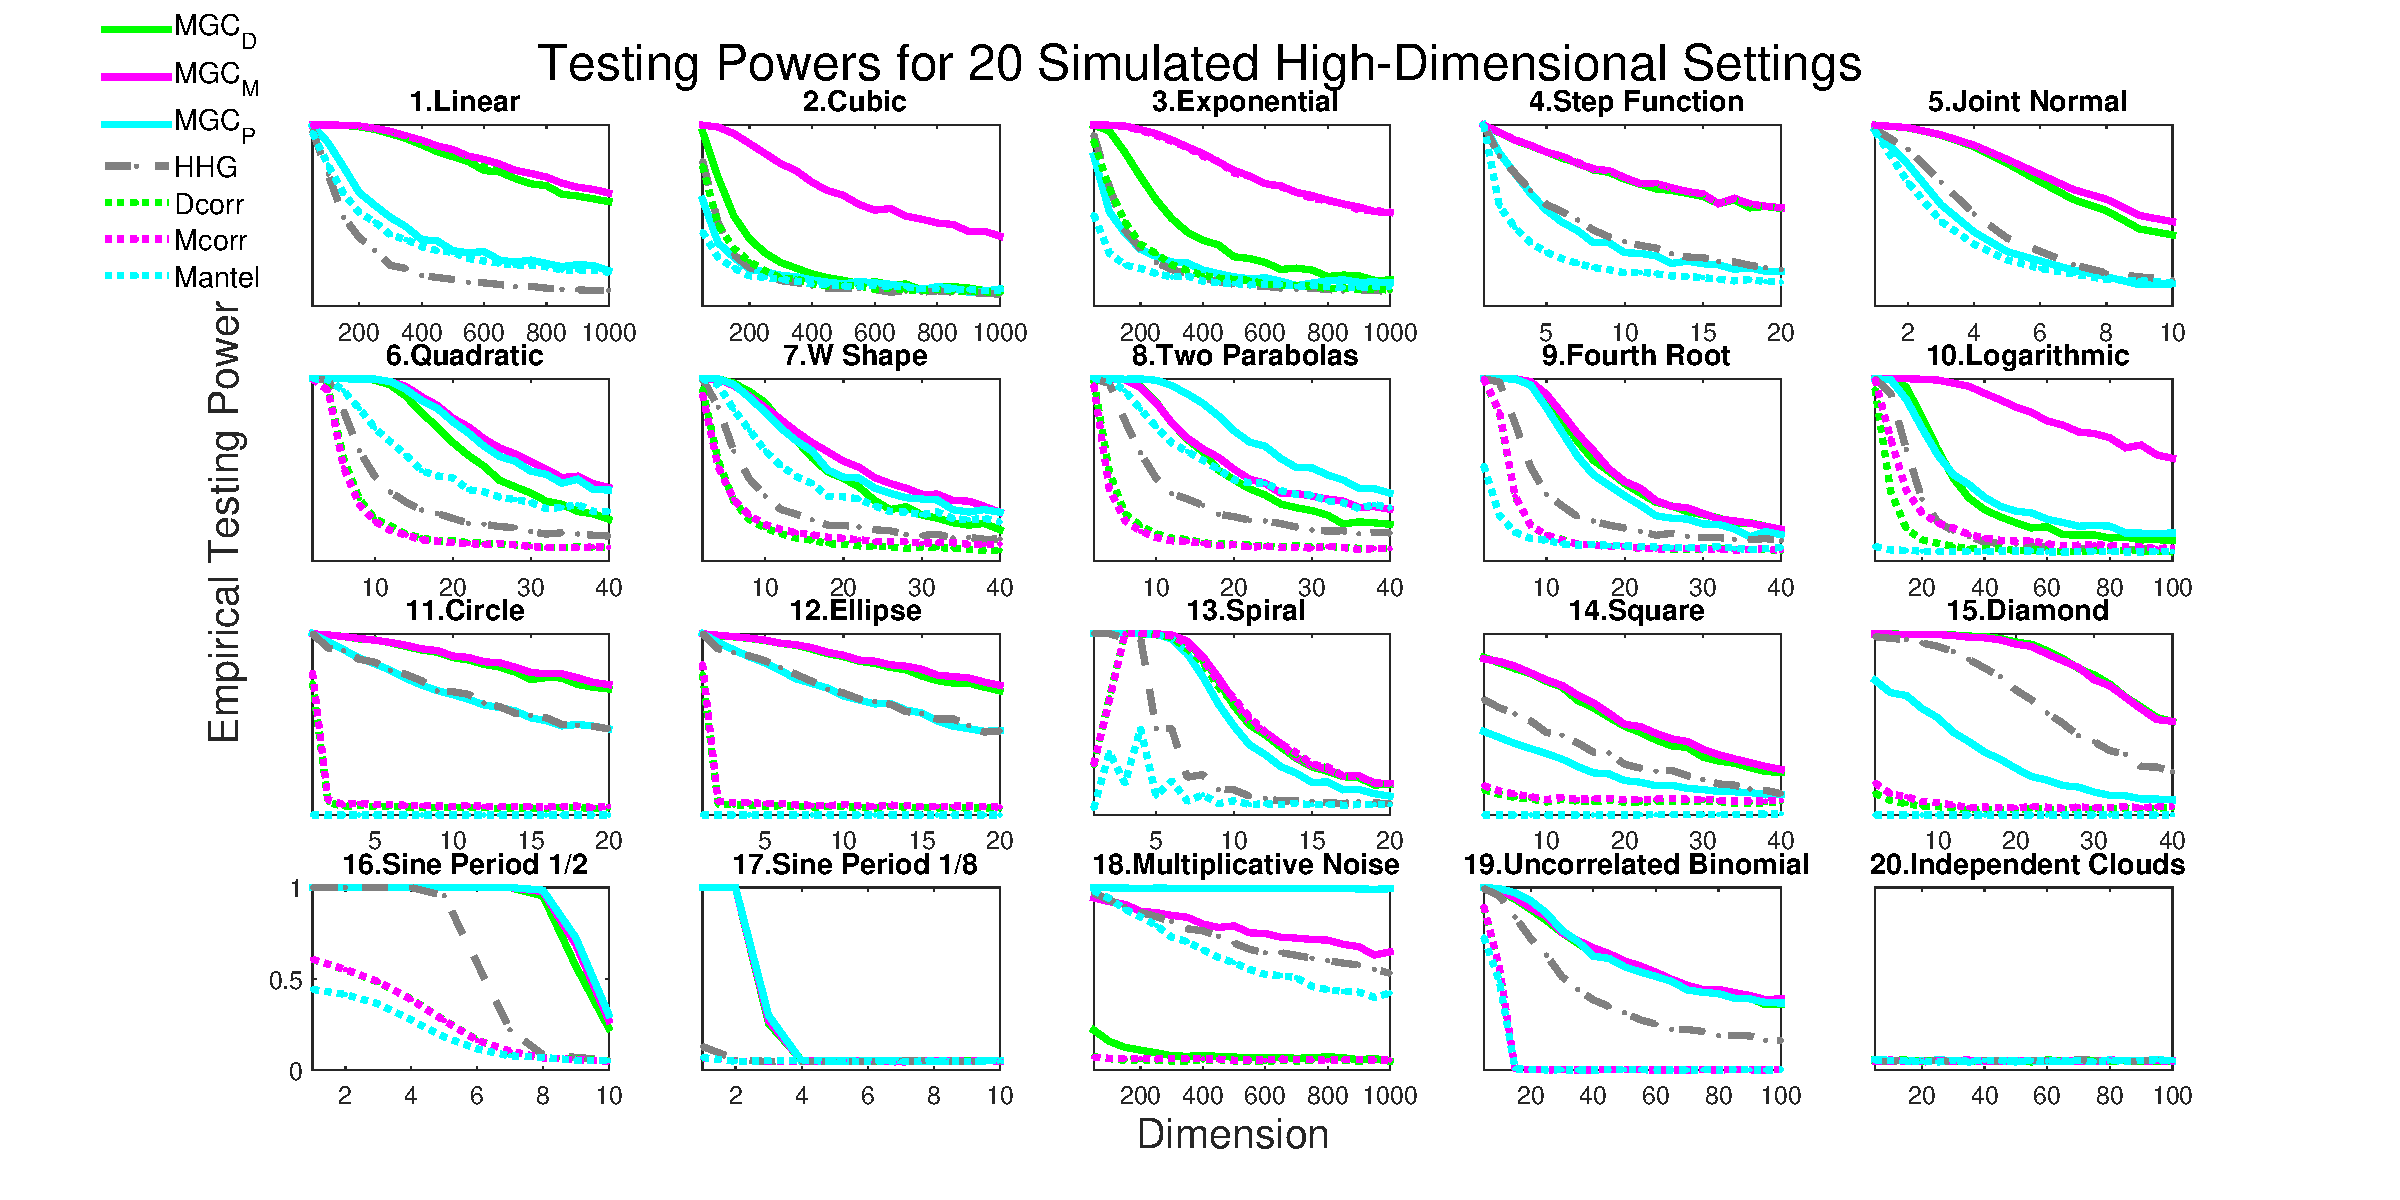
\includegraphics[width=1.0\textwidth,trim={0 0.5cm 4cm 0},clip]{Figures/FigHDPowerAll}
\caption{
Same as Figure~\ref{f:nD} in main text, but with all eight methods compared. Oracle and sample \Mgc~dominate the other approaches by being as powerful or more so for almost all simulations, regardless of the dimensionality. \Mgc~is always plotted ``on top'' of the global variants if there is overlap, therefore, some of the global variants are not always visible from the display.}
% * <stefaniejacinto@gmail.com> 2016-08-20T23:33:38.278Z:
%
% > if there is overlap
%
% What do you think about adding this phrase, for clarity?
%
% ^.
% \sd{its always on top though?}
\label{f:nDAll}
\end{figure}


\begin{figure}[htbp]
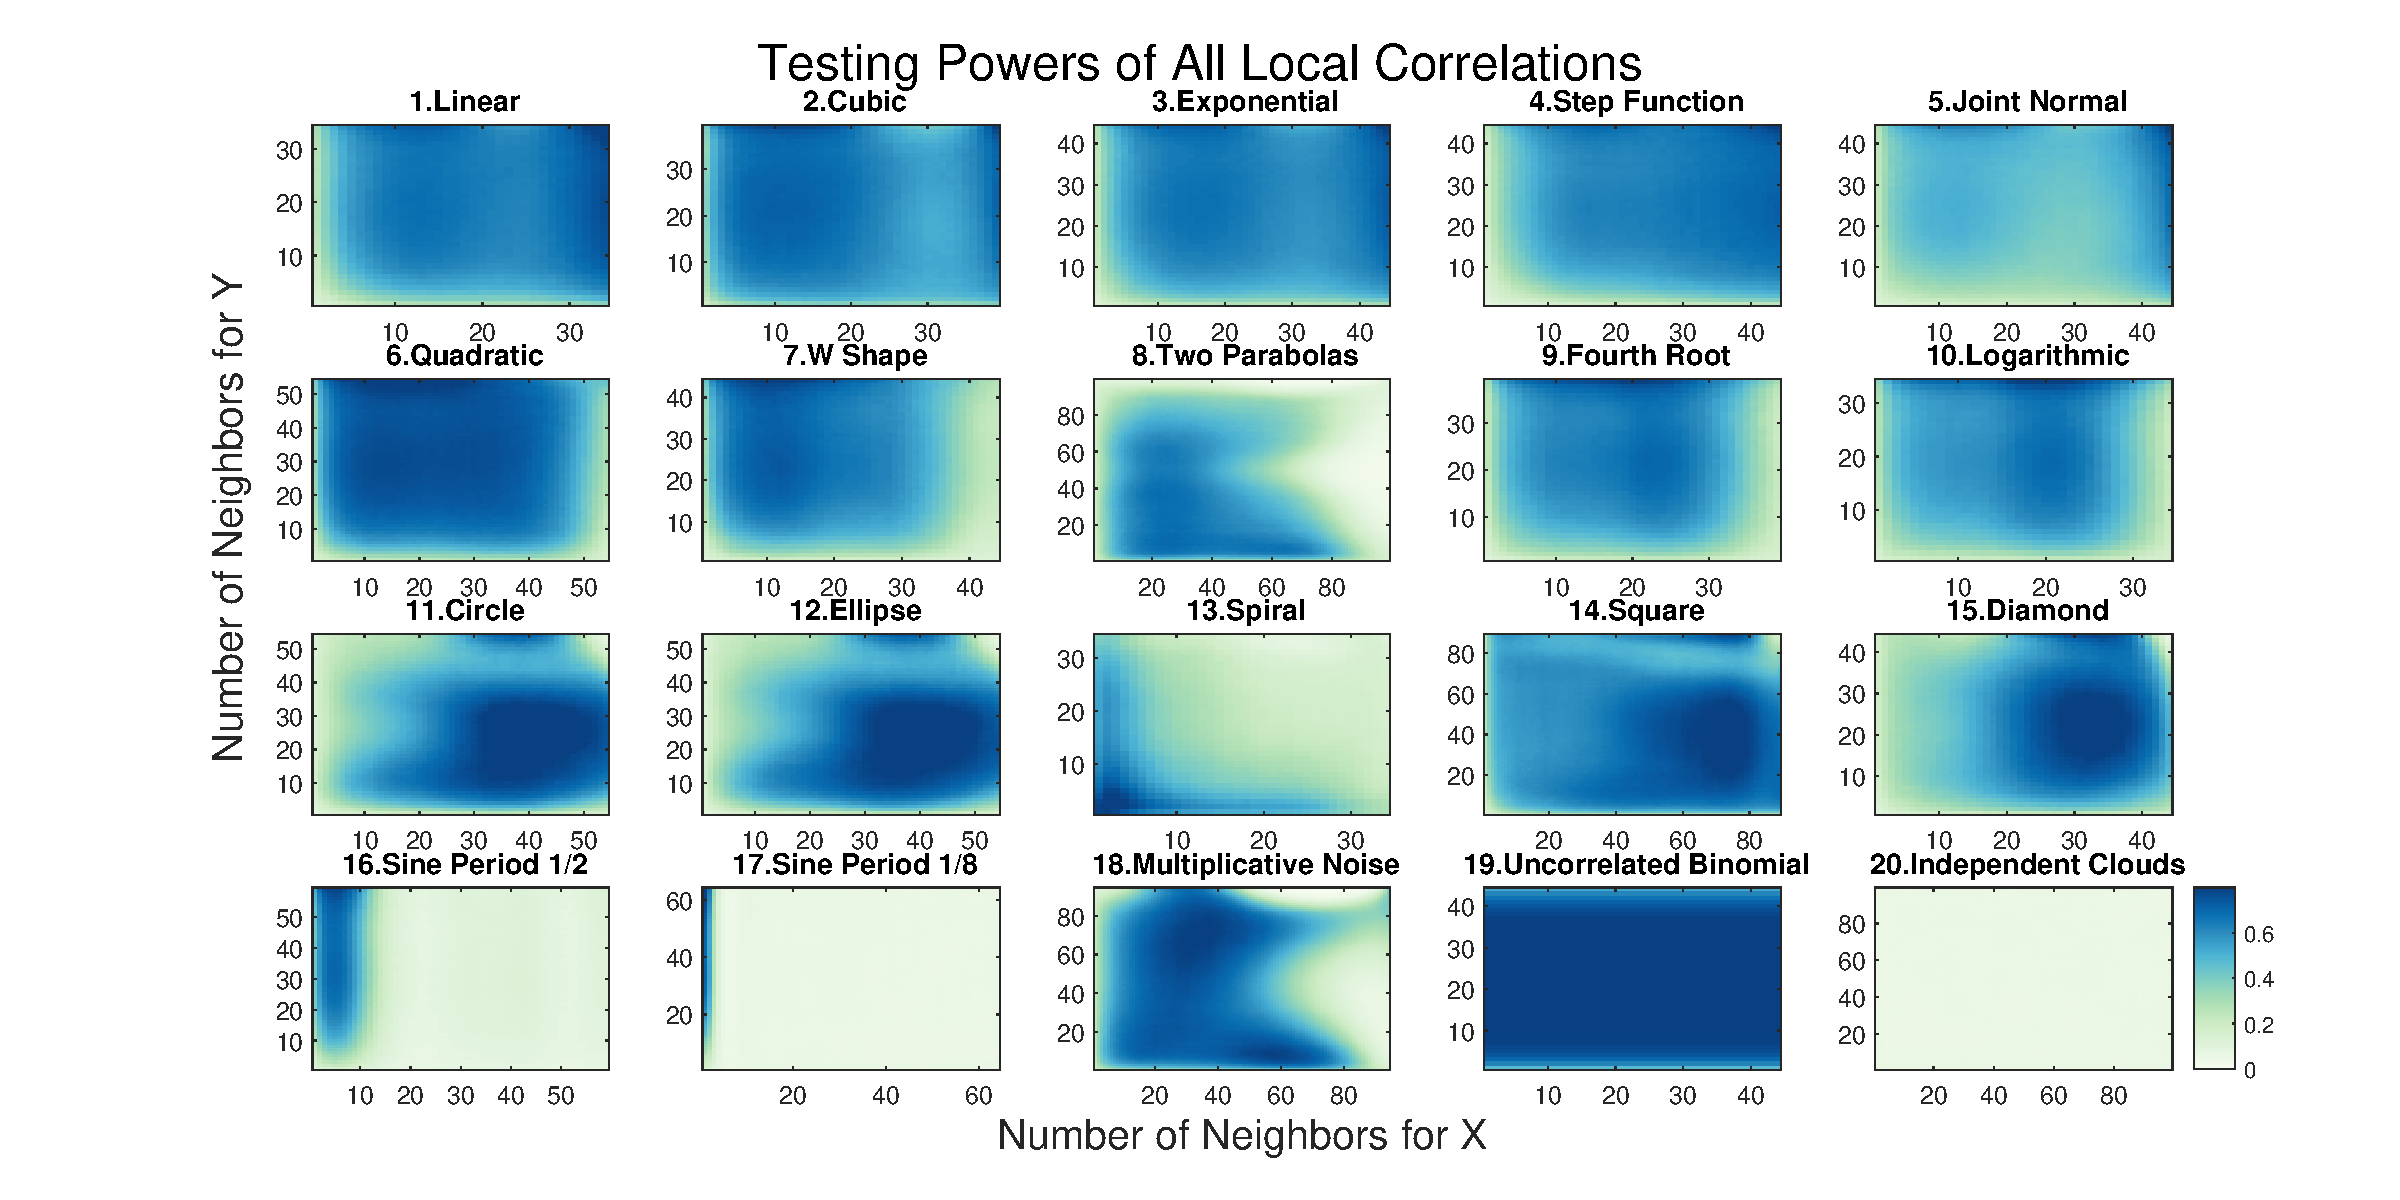
\includegraphics[width=1.0\textwidth,trim={3cm 0.5cm 2.5cm 0.5cm},clip]{Figures/Fig1DHeat}
\caption{Multiscale Power Maps indicating the influence of neighborhood size on \Mgc~testing power, for the one-dimensional simulations in Figure~\ref{f:1DAll}. For each simulation,  the sample size is $n=60$, and the significance level is $\alpha=0.05$. For the (nearly) linear settings, the global scales achieve optimal power.  However, for the other nonlinear dependence settings, local scales always outperform the global scale.}
\label{f:powermaps1}
\end{figure}

\clearpage
\section{Dependence Measures}
\label{appen:methods}

In this section, we review the \Mantel~test, distance correlation (\Dcorr), modified distance correlation (\Mcorr),  \Hhg, and \Mgc~along with some additional insights: for each global generalized correlation test (including \Mantel, \Dcorr, and \Mcorr), we show how to construct its multiscale variant, called \Mgcp, \Mgcd, and \Mgcm, respectively. For \Dcorr~and \Mcorr~, we show a slightly different but equivalent implementation from the original definitions, such that the resulting multiscale variants enjoy nicer theoretical properties and better empirical performances. Moreover, we show why our sample \Mgc~is tailored for Oracle \Mgcm~, but also provide general sample versions for \Mgcd~and \Mgcp.

\subsection{(Global) \Mantel~Test}
\label{appen:mantel}
Given the Euclidean distance matrices $\tilde{A}$ and $\tilde{B}$, let $A=\tilde{A}-\bar{a}$ and $B=\tilde{B}-\bar{b}$, where $\bar{a}=\frac{1}{n(n-1)}\sum_{i \neq j}^{n}(a_{ij})$ and similarly for $\bar{b}$.
The \Mantel~coefficient \cite{Mantel1967} is defined as
\begin{equation*}
\Mantel(X,Y)=\frac{\sum_{i \neq j}^{n}a_{ij}b_{ij}}{\sqrt{\sum_{i \neq j}^{n}a_{ij}^2 \sum_{i \neq j}^{n}b_{ij}^2}}.
\end{equation*}
Then the \Mantel~test is carried out by the permutation test.

Unlike distance correlation and \Hhg, the \Mantel~test is not consistent against all dependent alternatives, but it has been a very popular method in biology and ecology, possibly due to its simplicity and effectiveness. One can observe from Figure~\ref{f:1DAll} and ~\ref{f:nDAll} that global \Mantel~is sub-optimal relative to much more recently proposed tests (\Mantel~was proposed in 1967, \Dcorr~was not proposed until about 40 years later), and appears to be inconsistent for many dependencies. Nonetheless, Oracle \Mgcp~achieves comparable performance to other variants of \Mgc, which implies that \Mgcp~may be consistent with most, if not all dependent alternatives.
% * <stefaniejacinto@gmail.com> 2016-08-20T23:44:01.223Z:
%
% > achieves comparable performances to other variants of \Mgc, which implies that \Mgcp~may be consistent with most, if not all dependent alternatives.
%
% I corrected some prepositions. Please check to ensure intended meaning was preserved.
%
% ^.

\subsection{(Global) Distance Correlation}
\label{appen:dcorr}
Given two distance matrices $\tilde{A}$ and $\tilde{B}$ of the sample data $X$ and $Y$, the sample distance covariance is defined by doubly centering the distance matrices:
\begin{equation*}
\label{dcovEqu}
dcov(X,Y)=\frac{1}{n^2}\sum_{i,j=1}^{n}a_{ij}b_{ij},
\end{equation*}
where $A=H\tilde{A}H$, $B=H\tilde{B}H$ with $H=I_{n}-\frac{J_{n}}{n}$, $I_n$ the $n \times n$ identity matrix (ones on the diagonal, zeros elsewhere)  and $J_n$ the $n \times n$ matrix of all ones. The sample distance variance is defined as
\begin{align*}
dvar(X) &=\frac{1}{n^2}\sum_{i,j=1}^{n}a_{ij}^{2},\quad dvar(Y) =\frac{1}{n^2}\sum_{i,j=1}^{n}b_{ij}^{2},
\end{align*}
and the sample distance correlation equals
\begin{equation*}
\Dcorr(X,Y)=\frac{dcov(X,Y)}{\sqrt{dvar(X) \cdot dvar(Y)}}.
\end{equation*}

It is shown in \cite{SzekelyRizzoBakirov2007} that as $n \rightarrow \infty$, $\Dcorr(X,Y) \rightarrow \Dcorr(\mb{x},\mb{y}) \geq 0$, where $\Dcorr(\mb{x},\mb{y})$ denotes the population distance correlation between the underlying random variables $\mb{x}$ and $\mb{y}$. The population distance correlation is defined via the characteristic functions of $X$ and $Y$, in such a way that it is zero if and only if $\mb{x}$ and $\mb{y}$ are independent. Thus the sample distance correlation is a consistent statistic for testing independence, i.e., the testing power $\beta_{n}(\Dcorr(X,Y))$
converges to unity as $n$ increases, at any type $1$ error level $\alpha$. All of $dcov, dvar$, and \Dcorr~are always non-negative; and the consistency result assumes finite second moments of $\mb{x}$ and $\mb{y}$, which holds for a family of metrics not limited to the Euclidean distance \cite{Lyons2013}. Note that the \Dcorr~here equals the square of distance correlation in \cite{SzekelyRizzoBakirov2007}, but for ease of presentation the square naming is dropped here.

Alternatively, calculating the distance covariance by $A=H\tilde{A}$ and $B=\tilde{B}H$ gives the same statistic for distance covariance, i.e., instead of using doubly centered distance matrices, it is equivalent to singly center one distance matrix by row and the other distance matrix by column.
\begin{lem}
The distance covariance $dcov(X,Y)$ is the same under single centering (i.e., $A=H\tilde{A}$ and $B=\tilde{B}H$) and double centering (i.e., $A=H\tilde{A}H$ and $B=H\tilde{B}H$), where $\tilde{A}$ and $\tilde{B}$ are the Euclidean distance matrices of $X$ and $Y$, and $H$ is the centering matrix. 

Moreover, the permutation p-value of global \Dcorr~is the same under single centering and double centering, so is the testing power.
\end{lem}
Our \Mgcd~is in fact based on this single-centered \Dcorr, which is more advantageous than \Mgc~based on double-centered \Dcorr~(shown in Appendix~\ref{appen:mgc}). The proofs of all lemmas are in Appendix~\ref{appen:proofs}.



\subsection{(Global) Modified Distance Correlation}
\label{appen:mcorr}
In case of high-dimensional data where the dimension $D$ or $D_y$ increases with the sample size $n$, the sample distance correlation may no longer be appropriate. For example, even for independent Gaussian distributions, $\Dcorr(X,Y) \rightarrow 1$ as $D, D_y \rightarrow \infty$. Therefore \Dcorr~is a biased statistic at large $D$, which makes the interpretation of the actual test statistic much more difficult in practice, and may severely impair the testing power of sample \Dcorr~in high-dimensional simulations.

The modified distance correlation is proposed in \cite{SzekelyRizzo2013a} to tackle \Dcorr's bias in high-dimensional settings. Denote the Euclidean distance matrices as $\tilde{A}$ and $\tilde{B}$, and the doubly centered distance matrices as $A'$ and $B'$.  \Mcorr~defines $A$ by modifying the entries of $A'$ by
\[a_{ij} = \left\{
  \begin{array}{lr}
    a'_{ij}-\frac{\tilde{a}_{ij}}{n}, & \mbox{ if } i \neq j, \\
    \frac{1}{n}\sum_{j}\tilde{a}_{ij}-\frac{1}{n^2}\sum_{ij}\tilde{a}_{ij}, &\mbox{ if } i = j,
  \end{array}
\right.
\]
and  $B$ modifies the entries of $B'$ similarly.
The modified distance covariance is defined as
\begin{equation*}
mcov(X,Y)=\frac{n}{(n-1)^2(n-3)}\left(\sum_{i \neq j}^{n}a_{ij}b_{ij}-\frac{2}{n-2}\sum_{j=1}^{n}a_{jj}b_{jj}\right),
\end{equation*}
$mvar(X)$ and $mvar(Y)$ are defined similarly.

If $mvar(X) \cdot mvar(Y) \leq 0$, the modified distance correlation is set to $0$ (negativity can only occur when $n\leq 2$, equality can only happen in some special cases); otherwise it is defined as
\begin{equation*}
\Mcorr(X,Y)=\frac{mcov(X,Y)}{\sqrt{mvar(X) \cdot mvar(Y)}}.
\end{equation*}

It is shown in \cite{SzekelyRizzo2013a} that $\Mcorr(X,Y)$ is an unbiased estimator of the population distance correlation $\Dcorr(\mb{x},\mb{y})$ for all $D, D_y, n$; and \Mcorr~is approximately normal even if $D,D_y \rightarrow \infty$. Thus it is always of zero mean under independence, a consistent statistic for testing, and may work better than \Dcorr~for high-dimensional dependencies.

Similar to the alternative implementation of \Dcorr, we also use singly centered distance matrices for $A'$ and $B'$ in defining \Mcorr, which does not alter the theoretical advantages of the original \Mcorr. We further set $A_{ii}=B_{ii}=0$ for all $i$, which simplifies the expression of \Mcorr~and is still asymptotically equivalent for testing. 
Thus we use the single-centered \Mcorr~with zero diagonals for computational expediency and simplicity.


\subsection{Heller, Heller, \& Gorfine (\Hhg)}
\label{appen:hhg}

The \Hhg~statistic applies Pearson's chi-square test to ranks of distances within each column, and is shown to be better than many global tests including \Dcorr~under common nonlinear dependencies in \cite{GorfineHellerHeller2012, HellerGorfine2013}. Like \Dcorr~and \Mcorr, \Hhg~is distance-based and consistent, but not in the form of the generalized correlation coefficient; and like our \Mgc, it makes use of the rank information, but in a different manner.

Given the Euclidean distance matrices $\tilde{A}=\{\tilde{a}_{ij}\}$ and $\tilde{B}=\{\tilde{b}_{ij}\}$, we denote
\begin{align*}
H_{11}(i,j) &= \sum_{q=1,q\neq i,j}^{n}I(\tilde{a}_{iq} \leq \tilde{a}_{ij})I(\tilde{b}_{iq} \leq \tilde{b}_{ij}) \\
H_{12}(i,j) &= \sum_{q=1,q\neq i,j}^{n}I(\tilde{a}_{iq} \leq \tilde{a}_{ij})I(\tilde{b}_{iq} > \tilde{b}_{ij}) \\
H_{21}(i,j) &= \sum_{q=1,q\neq i,j}^{n}I(\tilde{a}_{iq} > \tilde{a}_{ij})I(\tilde{b}_{iq} \leq \tilde{b}_{ij}) \\
H_{22}(i,j) &= \sum_{q=1,q\neq i,j}^{n}I(\tilde{a}_{iq} > \tilde{a}_{ij})I(\tilde{b}_{iq} > \tilde{b}_{ij}),
\end{align*}
and the \Hhg~statistic is defined as
\begin{align*}
\Hhg(X,Y) &= \sum_{i=1,j\neq i}^{n} \frac{(n-2)(H_{12}(i,j)H_{21}(i,j)-H_{11}(i,j)H_{22}(i,j))^2}{H_{1 \cdot}(i,j)H_{2 \cdot}(i,j)-H_{\cdot 1}(i,j)H_{\cdot 2}(i,j)},
\end{align*}
where $H_{1 \cdot}=H_{11}+H_{12}$, $H_{2 \cdot}=H_{21}+H_{22}$, $H_{\cdot 1}=H_{11}+H_{21}$, and $H_{\cdot 2}=H_{12}+H_{22}$. Thus \Hhg~is structurally different from all previous distance-based correlations, and cannot be conveniently expressed by Equation~\ref{generalCoef}.

The permutation test using the \Hhg~statistic is consistent against all dependent alternatives. In our numerical simulations, \Hhg~has relatively low power  when testing against high-dimensional and noisy linear dependencies, but is often more advantageous than global correlations under nonlinear dependencies, which makes it a strong competitor in general. 
$\Hhg$ is invariant not only with respect to rescaling of the distances $\delta_x$ and $\delta_y$, but to general monotone transformations.

\subsection{Multiscale Generalized Correlation (\Mgc)}
\label{appen:mgc}
For any generalized correlation coefficient, its local correlations can be directly implemented as in Equation~\ref{localCoef}, by plugging in the respective $a_{ij}$ and $b_{ij}$ from Equation~\ref{generalCoef} and rank-truncating  the distance matrices  as in Equation~\ref{localCoef2}. 

In particular, \Mantel~sets $a_{ij}$ and $b_{ij}$ as the respective entries of $\tilde{A}$ and $\tilde{B}$ (the Euclidean distances). \Dcorr~lets $a_{ij}$ and $b_{ij}$ be the respective matrix entries of $A$ and $B$ (the doubly centered distance matrices), then the sample means $\bar{a}$ and $\bar{b}$ are automatically $0$. \Mcorr~slightly modifies $a_{ij}$ and $b_{ij}$ of \Dcorr~to adjust their high-dimensional bias. 

As discussed already, our \Mgcd~and \Mgcm~are based on single centering throughout, not only because single centering is equivalent to double centering for the global correlation, but also because single centering is consistent in preserving ranks while double centering is not, e.g., the ranks by sorting $\tilde{A}$ within each column are exactly the same as the column ranks of $H\tilde{A}$, which are different from the column ranks of $H\tilde{A}H$. 

Note that we defined the rank-truncated comparisons differently for $\mt{a}_{ij}^k$ and $\mt{b}_{ij}^l$: $\mt{a}_{ij}^k$ is defined based on ranks within each column, while $\mt{b}_{ij}^l$ is defined based on ranks within each row. By doing so, the ranks are consistent between $\tilde{Z}$ and $Z$ for either $Z=A,B$, and the resulting local correlations are always symmetric even if $A$ and $B$ are not symmetric.

\begin{lem}
Each local correlation $\G^{kl}$ is always symmetric regardless of the symmetry of $A$ or $B$. Namely for any $k,l$, 
\begin{align*}
\G^{kl}(X,Y)=\G^{lk}(Y,X).
\end{align*}
Furthermore, the column ranks of $\tilde{A}$ are preserved in $A$ under single centering but not double centering; similarly the row ranks of $\tilde{B}$ are preserved in $B$ under single centering.
\end{lem}
Therefore local correlations are more faithful in excluding far-away observations that exhibit insignificant dependency, when \Mgc~is implemented by single centering.

Generally, there are a total of $\max(R(a_{ij})) \times \max(R(b_{ij}))$ local correlations, which equals $n^2$ when there exists no repeating values of \mbx~or \mby. Note that we use minimal ranks in sorting when ties occur, which guarantees that all local correlations are indexed consecutively. Alternatively, one may add a very small amount of white noise to break all ties, like in our real data experiment.

Among all possible local correlations, Oracle \Mgc~picks the optimal local correlation $\G^{*}$ by maximizing the power map. The optimal scales always exist,  are distribution dependent, and are often non-unique. Among all local correlations, it suffices to exclude $\G^{1l}$ and $\G^{k1}$: since $\G^{1l}=\G^{k1}=\G^{11}$, they do not include any neighbor other than each observation itself, merely count the diagonal terms in the distance matrices, and will not be selected as optimal after all.

Our sample \Mgc~provides an estimate $\hat{\G}^{*}$ of the optimal local correlation, by identifying significant scales in the local correlation map rather than the power map (details in algorithm~\ref{alg:sample_mgc}). However, as \Dcorr~is biased, its' local correlations are also biased (the expectations may not be $0$ under independence), such that significant scales cannot be easily determined by the the magnitude of each local statistic; while the unbiased-ness of \Mcorr~allows its' local correlations to be compared more meaningfully, and a test statistic much larger than $0$ always implies significant local correlation, which allows a fast and valid sample \Mgc~statistic to be tailored for \Mgcm~. 

Note that a general sample estimation technique exists for \Mgcd~and \Mgcp~as well: instead of estimating an optimal test statistic within the local correlation map, one may estimate the optimal p-value from the p-value map (e.g., by significant and monotone p-values), by treating the estimated p-value as a test statistic and running the permutation test again to compute the true p-value for the sample version of any multiscale variant. This technique is immune to the bias of local correlations, and is suggested by Heller et al. (2016) \cite{heller2016consistent}. Since this general technique requires more random permutations and is much slower, and does not offer any more theoretical or numerical advantages in testing, in this paper we stick to our current sample \Mgc~method for \Mcorr~only and do not delve into this general technique.


\section{\Mgc~Algorithms and Testing Procedures}
\label{appen:tests}
In this section, we elaborate on the algorithms for computing all local correlations, Oracle and sample \Mgc, the optimal scale estimation, as well as the testing power and p-value computations.

Five algorithms are presented in Appendix~\ref{appen:algorithms}: Algorithm~\ref{alg:1scale} directly computes the local correlation coefficient at a given scale $(k,l)$, for a given choice of the global correlation coefficient.
Algorithm~\ref{alg:all_scales} provides an efficient method to compute all local correlations simultaneously, in the same running time complexity as computing one local correlation. 
Algorithm~\ref{alg:power} computes the testing power of all local statistics using a known or estimated joint distribution, which can be used to accurately determine the optimal scales and test statistic for Oracle \Mgc~by simulations. 
Algorithm~\ref{alg:sample_mgc} is the sample \Mgc~algorithm, which provides an estimate of the Oracle \Mgc~among all local correlations. It finds a sufficiently large region with significantly large and monotonically changing local correlations, and uses a large local correlation within the region as the sample \Mgc~statistic; otherwise it uses the global correlation. %More detailed discussions regarding sample \Mgc~is offered in Appendix~\ref{appen:diss}.
Algorithm~\ref{alg:pval} computes the p-values of all local correlation by the random permutation test, which also includes the p-value computation and the optimal scale estimation by sample \Mgc.

\subsection{Algorithms}
\label{appen:algorithms}
All algorithms are implemented in Matlab and R with the algorithm shown below. For ease of presentation, we assume there are no repeating observations of \mbx~or \mby, and assume \Mcorr~is the global correlation.

\begin{algorithm}
\caption{Compute local test statistic for a given scale. This algorithm runs in $O(n^2)$ once the rank information is provided, which is suitable for \Mgc~computation if an optimal scale is already estimated. But it would take $O(n^4)$ if used to compute all local correlations. Note that for the default \Mgc~implementation by single centering, the centering function centers $\tilde{A}$ by column and $\tilde{B}$ by row, and the sorting function sorts $\tilde{A}$ within column and $\tilde{B}$ within row.}
\label{alg:1scale}
\begin{algorithmic}[1]
\Require A pair of distance matrices $(\tilde{A},\tilde{B}) \in \Real^{n \times n} \times \Real^{n \times n}$, and the given local scale $(k,l) \in \mathbb{N} \times \mathbb{N}$.
\Ensure The local correlation coefficient $\G^{kl} \in [-1,1]$ at the given $(k,l)$.
\Function{LocalCorr}{$\tilde{A}$,$\tilde{B}$,$k$,$l$}
\State Initialize $\G^{kl}$, $V^{A}_{k}$, $V^{B}_{l}$, $E^{A}_{k}$, $E^{B}_{l}$ at $0$.
\Linefor{$Z:=A,B$}{$R^{Z}=\textsc{Sort}(\tilde{Z})$} \Comment{sort distances}
\Linefor{$Z:=A,B$}{$Z=\textsc{Center}(\tilde{Z})$}  \Comment{center distance matrices}
%\State $R^{B}=\textsc{Transpose}(R^{B})$ \Comment{row-wise ranks are used for second data}
%\State $B=\textsc{Transpose}(B)$ \Comment{row-wise ranks are used for second data}

\For{$i,j:=1,\ldots,n$}
\State $\G^{kl} \rto \G^{kl}+A_{ij}B_{ij}\mb{I}(R^{A}_{ij} \leq k)\mb{I}(R^{B}_{ij} \leq l)$ \Comment{update un-centered local distance covariance}
\Linefor{$Z:=A,B$}{$V^{Z}_{k} \rto V^{Z}_{k}+Z_{ij}^2\mb{I}(R^{Z}_{ij} \leq k)$} \Comment{update local distance variances}
\Linefor{$Z:=A,B$}{$E^{Z}_{k} \rto E^{Z}_{k}+Z_{ij}\mb{I}(R^{Z}_{ij} \leq k)$} \Comment{update sample means}
\EndFor

\State $\G^{kl} \rto \left(\G^{kl}-E^{A}_{k}E^{B}_{l}/n^2\right)/\sqrt{\left(V^{A}_{k}-{E^{A}_{k}}^2/n^2\right) \left(V^{B}_{l}-{E^{B}_{l}}^2/n^2\right)}$ \Comment{center and normalize} 
% the local covariances}

\EndFunction
\end{algorithmic}
\end{algorithm} 

\begin{algorithm}
\caption{Compute local test statistic for all scales in $O(n^2 \log n)$. Once the distances are sorted, this algorithm computes all local correlations in $O(n^2)$. An important observation is that each product $a_{ij}b_{ij}$ is included in $\G^{kl}$ if and only if $(k,l)$ satisfies $k\leq R(a_{ij})$ and $l\leq R(b_{ij})$, so it suffices to iterate through $a_{ij}b_{ij}$ for $i,j=1,\ldots,n$, and add the product simultaneously to all $\G^{kl}$ whose scales are no more than $(R(a_{ij}),R(b_{ij}))$. To achieve the above, we iterate through each product, add it to $\G^{kl}$ at $(k,l)=(R(a_{ij}),R(b_{ij}))$ only (so only one local scale is accessed for each operation); then add up adjacent $\G^{kl}$ for $k,l=1,\ldots,n$. The same applies to all local covariances, variances, and expectations.} %Thus all local correlations can be computed in $O(n^2)$, which has the same running time complexity as the global distance correlation. There are two additional overheads: sorting the distance matrices column-wise takes $O(n^2 \log n)$, and properly centering the distance matrices takes $O(n^2)$.}
\label{alg:all_scales}
\begin{algorithmic}[1]
\Require A pair of distance matrices $(\tilde{A},\tilde{B}) \in \Real^{n \times n} \times \Real^{n \times n}$.
\Ensure All local correlation coefficients $\{\G^{kl}\} \in [-1,1]^{n \times n}$ for $k,l=1,\ldots,n$.
\Function{LocalCorr}{$\tilde{A}$,$\tilde{B}$}
\State Initialize $C$ as a zero matrix of size $n \times n$; $V^{A}$, $V^{B}$, $E^{A}$, $E^{B}$ as zero vectors of size $n$.
\Linefor{$Z:=A,B$}{$R^{Z}=\textsc{Sort}(\tilde{Z})$}
%\State $R^{B}=\textsc{Transpose}(R^{B})$ 
\Linefor{$Z:=A,B$}{$Z=\textsc{Center}(\tilde{Z})$}

\For{$i,j:=1,\ldots,n$} \Comment{iterate through all local scales to calculate each term} 
\State $k \rto R^{A}_{ij}$
\State $l \rto R^{B}_{ij}$
\State $\G^{kl} \rto \G^{kl}+A_{ij}B_{ij}$
\State $V^{A}_{k} \rto V^{A}_{k}+A_{ij}^2$
\State $V^{B}_{l} \rto V^{B}_{l}+B_{ij}^2$
\State $E^{A}_{k} \rto E^{A}_{k}+A_{ij}$
\State $E^{B}_{l} \rto E^{B}_{l}+B_{ij}$
\EndFor

\For{$k:=1,\ldots,n-1$} \Comment{iterate through each scale again and add up adjacent terms} 
\State $\G^{1, k+1} \rto \G^{1, k}+\G^{1, k+1}$
\State $\G^{k+1,1} \rto \G^{k+1,1}+\G^{k+1,1}$
\Linefor{$Z:=A,B$}{$V^{Z}_{k+1} \rto V^{Z}_{k}+V^{Z}_{k+1}$}
\Linefor{$Z:=A,B$}{$E^{Z}_{k+1} \rto E^{Z}_{k}+E^{Z}_{k+1}$}
\EndFor

\For{$k,l:=1,\ldots,n-1$} 
\State $\G^{k+1,l+1} \rto \G^{k+1,l}+\G^{k,l+1}+\G^{k+1,l+1}-\G^{k,l}$
\EndFor

\For{$k,l:=1,\ldots,n$} 
\State $\G^{kl} \rto \left(\G^{kl}-E^{A}_{k}E^{B}_{l}/n^2\right)/\sqrt{\left(V^{A}_{k}-{E^{A}_{k}}^2/n^2\right) \left(V^{B}_{l}-{E^{B}_{l}}^2/n^2\right)}$
\EndFor
\EndFunction
\end{algorithmic}
\end{algorithm}

\begin{algorithm}
\caption{Compute power for all local tests. This algorithm computes the  power of all local correlations. By repeatedly simulating samples by the joint distribution $f_{xy}$, sample data of size $n$ under the null and the alternative are generated for $r$ Monte-Carlo replicates. Then all local correlations under the null and the alternative hypotheses are computed by Algorithm~\ref{alg:all_scales}, followed by estimating the testing power at each local correlation. The optimal scales of Oracle \Mgc~can be found by all scales that maximizes the power. The running time is $O(rn^2 \log n)$. In the simulations we use $r=2$,$000$ MC replicates to estimate the optimal scale, and another $r=10$,$000$ MC replicates to estimate the power. This algorithm can be similarly adapted to training data, for which the alternative statistic can be computed from the training data while the null statistic can be computed by permutation. Note that power computation for sample \Mgc~or other benchmarks follows from the same algorithm, by plugging in the respective test statistic in the first loop without the optimal scale computation. }
\label{alg:power}
\begin{algorithmic}[1]
\Require A joint distribution $f_{xy}$, the sample size $n$, the number of MC replicates $r$, and the type $1$ error level $\alpha$.
\Ensure The power matrix $\beta \in [0,1]^{n \times n}$ for all local correlations, and the \Mgc~optimal scale $(k^{*},l^{*}) \in \mathbb{N} \times \mathbb{N}$.
\Function{TestingPower}{$f_{xy}$,$n$, $r$,$\alpha$}
\For{$j:=1,\ldots,r$}
\Linefor{$i:=[n]$}{$(X^{1}_{i},Y^{1}_{i}) \stackrel{iid}{\sim} f_{xy}$, $X^{0}_{i} \stackrel{iid}{\sim} f_{x}$, $Y^{0}_{i} \stackrel{iid}{\sim} f_{y}$} 
\Linefor{$Z:=A,B$}{$\tilde{Z}_{1}=\textsc{Dist}(Z_{1})$, $\tilde{Z}_{0}=\textsc{Dist}(Z_{0})$} 
\State $\{\G^{kl}_{1}\}[j]=\textsc{LocalCorr}(\tilde{A}_{1},\tilde{B}_{1})$ \Comment{calculate all local correlations under the alternative}
\State $\{\G^{kl}_{0}\}[j]=\textsc{LocalCorr}(\tilde{A}_{0},\tilde{B}_{0})$ \Comment{calculate all local correlations under the null}
\EndFor

\For{$k,l:=1,\ldots,n$}
\State $\omega_{\alpha} \rto \textsc{Cdf}_{1-\alpha}(\G^{0}_{kl}[j],j \in [r])$ \Comment{get the critical value by the empirical distributions}
\State $\beta_{kl} \rto \sum_{j=1}^{r}(\G^{1}_{kl}[j]>\omega_{\alpha}) / r$ \Comment{compute the power map}
\EndFor
\State $(k^{*},l^{*}) \rto \arg_{k,l}\max(\{\beta_{kl}\})$ \Comment{compute the optimal local scales}
\EndFunction
\end{algorithmic}
\end{algorithm}

\begin{algorithm}
\caption{Compute the sample \Mgc~test statistic. By default, the global distance correlation is used. But if there exists a sufficiently large region such that all correlations within the region are monotonically increasing or decreasing along the row or column, and are significantly large (governed by the threshold $\epsilon$ computed from negative local correlations), we take a large correlation within the monotone and significant region. The running time is $O(n^2)$.}
\label{alg:sample_mgc}
\begin{algorithmic}[1]
\Require All local statistics $\{\G^{kl}\} \in \Real^{n \times n}$.
\Ensure The sample \Mgc~statistic $\hat{\G}^{*} \in \Real$.
\Function{SampleMGC}{$\{\G^{kl}\}$}
\State $\epsilon \rto \sum_{\G^{kl}<0} (\G^{kl})^2 / \sum_{\G^{kl}<0} 1$ \Comment{variance of all negative local correlations away from $0$}
\State $\epsilon \rto 3.5\max\{0.01,\sqrt{\epsilon}\}$ \Comment{threshold for identifying significant local correlations}
\State $\hat{\G}^{*} \rto \G^{nn}$ \Comment{use the global correlation by default}

%\State $R=\textsc{Connected}(\G^{kl}>\epsilon)$ \Comment{a binary matrix indicating largest connected component}
\If{$\sum_{k,l} R_{kl} \geq 2n$} \Comment{proceed when the region is sufficiently large}
\State $R = \textsc{Monotone}(\{\G^{kl}\},R)$ \Comment{check monotonically changing local correlations} 
\State $\Omega \rto \arg_{k,l}\{(\G^{kl}\geq \max_{R_{kl}=1} \G^{kl}) \cap (R_{kl}=1)\}$ \Comment{scale with largest correlation in $R$}
\State $\gamma=\textsc{Ceiling}(0.1n)$
\For{$(k',l') \in \Omega$}
\State $\theta_{1} \rto \min_{k \in [k'-\gamma,k'+\gamma]}\{\G^{kl'}\}$ \Comment{minimal correlation at given column along nearby rows}
\State $\theta_{2} \rto \min_{l \in [l'-\gamma,l'+\gamma]}\{\G^{k'l}\}$ \Comment{minimal correlation at given row along nearby columns}
\State $\theta \rto \max\{\theta_{1},\theta_{2}\}$
\Lineif{$\theta > \hat{\G}^{*}$}{ $\hat{\G}^{*} \rto \theta$}
\EndFor
\EndIf
\EndFunction
\end{algorithmic}
\
\
\begin{algorithmic}[1]
\Require All local statistics $\{\G^{kl}\} \in \Real^{n \times n}$, and a binary matrix $R \in \Real^{n \times n}$ for significant correlations.
\Ensure A binary matrix $R' \in \Real^{n \times n}$ indicating monotone significant local correlations.
\Function{Monotone}{$\{\G^{kl}\},R$}
\State $R_{r} = \textsc{Diff}(\{\G^{kl}\},1)$ \Comment{correlation change along the row}
\State $R_{c} = \textsc{Diff}(\{\G^{kl}\},2)$ \Comment{correlation change along the column}
\State $R[1] \rto (R_{r} \geq 0)$ \Comment{a binary matrix indicating increasing correlations along the row} 
\State $R[2] \rto (R_{r} \leq 0)$ \Comment{a binary matrix indicating decreasing correlations along the row} 
\State $R[3] \rto (R_{c} \geq 0)$ \Comment{repeat for column correlation changes} 
\State $R[4] \rto (R_{c} \leq 0)$
\For{i:=1,\ldots,4}
\State $R[i] \rto \textsc{Connected}(R[i] \cap R)$ \Comment{a binary matrix for largest connected component}
\State $R' \rto R' \cup R[i]$
\EndFor
\EndFunction
\end{algorithmic}
\end{algorithm}

\begin{algorithm}
\caption{Compute p-value  Sample \Mgc, and estimate the optimal scales. This algorithm uses a permutation test with $r-1$ random permutations, requiring $O(rn^2 \log n)$. Specifically, it computes the multiscale test-statistic map from the real data and from $r-1$ resamples.   For each, it then computes $c^{kl}_0$, which is the ``optimal'' test statistic.  The p-value is estimated using the permutation test.  Then, it estimates the optimal scales by computing the p-values for all scales, and letting the largest rectangle with local p-values less than or equals to the p-value of sample \Mgc.  In the real data experiment we always set $r=10$,$000$. Note that the p-value computation for any other global generalized correlation coefficient follows from the same algorithm by replacing sample \Mgc~with the respective test statistic.
}
\label{alg:pval}
\begin{algorithmic}[1]
\Require A pair of distance matrices $(\tilde{A},\tilde{B}) \in \Real^{n \times n} \times \Real^{n \times n}$, the number of permutations $r$.
\Ensure The p-value matrix $P \in [0,1]^{n \times n}$ for all local correlations, the p-value $p \in [0,1]$ for sample \Mgc, and estimated \Mgc~optimal scale $(\hat{k}^{*},\hat{l}^{*}) \in \mathbb{N} \times \mathbb{N}$.
\Function{PermutationTest}{$\tilde{A}$,$\tilde{B}$,$r$}
\State $\{\G^{kl}\}=\textsc{LocalCorr}(\tilde{A},\tilde{B})$ \Comment{calculate the observed local correlations}
\State $\hat{\G}^{*}=\textsc{SampleMGC}(\{\G^{kl}\})$ \Comment{sample \Mgc~statistic}
\For{$j:=1,\ldots,r$}
\State $\pi=\textsc{RandPerm}(n)$ \Comment{generate a random permutation of size $n$} 
\State $\{\G^{kl}_{0}\}[j]=\textsc{LocalCorr}(\tilde{A},\tilde{B}(\pi,\pi))$ \Comment{calculate the permuted test statistics}
\State $\hat{\G}^{*}_{0}[j]=\textsc{SampleMGC}(\{\G^{kl}_{0}\}[j])$ \Comment{calculate the permuted sample \Mgc}
\EndFor

\Linefor{$k,l:=1,\ldots,n$}{$P_{kl} \rto \sum_{j=1}^{r}(\G^{kl} \leq \G^{kl}_{0}[j])/r$} \Comment{the p-value map}
\State $p \rto \sum_{j=1}^{r}(\hat{\G}^{*} \leq \hat{\G}^{*}_{0}[j])/r$  \Comment{the p-value map for sample \Mgc}
\State $(\hat{k}^{*},\hat{l}^{*}) = \textsc{LargestRectangle}(P\leq p)$ \Comment{estimate the optimal scales}
\EndFunction
\end{algorithmic}
\end{algorithm}

\clearpage


\section{Proofs}
\label{appen:proofs}
\begin{appThm}
$\beta_n(\Mgc_t) \rightarrow 1$ as $n \to \infty$ for all $f_{xy}$ in $\mc{F}_t$.
In words, Oracle \Mgc~is consistent with all dependent alternatives for which its global counterpart is consistent. 
\end{appThm}
\begin{proof}
Since $\beta_n(\Mgc_t)=\underset{kl}{\max}\{\beta_n(\G_t^{kl})\}$, for any $f_{xy}$ the power of \Mgc~satisfies
\begin{equation*}
\beta_n(\Mgc_t) \geq \beta_n(\G_t)
\end{equation*}
at any type $1$ error level $\alpha$. So $\beta_n(\Mgc_t) \rightarrow 1$ if $\beta_n(\G_t) \rightarrow 1$.
% 
Therefore $\beta_n(\Mgc_t) \rightarrow 1$ for all $f_{xy}$ in $\mc{F}_t$. In particular, \Mgcd~and \Mgcm~are consistent with all alternatives satisfying certain regularity conditions, because \Dcorr~and \Mcorr~are consistent by \cite{SzekelyRizzoBakirov2007, SzekelyRizzo2013a}. 
\end{proof}

\begin{appThm}
If $\mb{x}$ is linearly dependent on $\mb{y}$, then for any $n$ it always holds that
\begin{equation}
\beta_n(\Mgc_t) = \beta_n(\G_t).
\end{equation}
In words, the global scale is the optimal scale for Oracle \Mgc~for linearly dependent data.
\end{appThm}

\begin{proof}
To show that \Mgc~is equivalent to the global correlation coefficient, it suffices to show the p-value of $\G^{kl}_t$ is always no less than the p-value of $\G_t$ for all $k,l$ and any $n$ under linear dependence. In the permutation test, the p-value equals the percentage of permutations such that the permuted test statistic is no less than the observed test statistic, so it suffices to compare the number of ``significant'' permutations for $\G_t$ and $\G^{kl}_t$.

Without loss of generality, we assume all of $a_{ij}$, $b_{ij}$, $a_{ij}^{k}$, and $b_{ij}^{l}$ are of zero-mean, as simple centering or not does not affect the p-value; and we assume \Dcorr~with double centering are used, as Lemma~\ref{lem1} shows that double centering and simple centering yield the same testing power and p-value.

Under linear dependency, by Cauchy-Schwarz inequality the distance correlation satisfies
\begin{align*}
& dcov(X,Y) = \sqrt{dvar(X) \cdot dvar(Y)} \quad\Rightarrow\quad 1=\G(X, Y) \geq \G(X, Y_{\pi})
\end{align*}
for any permutation $\pi$, where the equality holds if and only if $X$ is a scalar multiple of $Y_{\pi}$, i.e., $a_{ij}=b_{\pi^{-1}(i) \pi^{-1}(j)}$ for all $i,j$, where $\pi^{-1}(\cdot)$ denotes the inverse permutation. %It follows that the p-value of $\G$ is $0$, which is at the minimal.

Thus for the global correlation, there only exist permutations such that the permuted test statistic equals the observed test statistic. However, for all those ``significant'' permutations for $\G$, they are also ``significant'' for each $\G^{kl}$, i.e., $a_{ij}^{k}=b_{\pi^{-1}(i) \pi^{-1}(j)}^{l}$ if $a_{ij}=b_{\pi^{-1}(i) \pi^{-1}(j)}$, such that $\G^{kl}(X, Y)=\G^{kl}(X, Y_{\pi})$; and there may exist other ``significant'' permutations such that $\G^{kl}(X, Y) \leq \G^{kl}(X, Y_{\pi})$.

Therefore the number of ``significant'' permutations for $\G^{kl}$ at least equals those for $\G$ under linear dependency, and the p-value of $\G^{kl}$ cannot be less than the p-value of $\G$, in which case the global correlation is optimal for \Mgc. 
\end{proof}

\begin{appThm}
There exists $f_{xy}$ and $n$ such that
\begin{equation}
\beta_n(\Mgc_{t}) \geq \beta_n(\G^{k,l}_{t}) > \beta_n(\G_{t}).
\end{equation}
In words, for finite samples, many different scales of \Mgc~can be better than the global scale under certain nonlinear dependency.
\end{appThm}

\begin{proof}
We give a simple discrete example of $f_{xy}$ at $n=7$, such that the p-value of \Mgcm~is strictly lower than the p-value of \Mcorr.

Suppose under the alternative, each pair of observation $(\mb{x},\mb{y})$ is sampled as follows:
\begin{align*}
\mb{x} &\in \left\{-1,-\frac{2}{3},-\frac{1}{3},0,\frac{1}{3},\frac{2}{3},1\right\} \mbox{ without replacement}, \\
\mb{y} &= \mb{x}^2,
\end{align*}
which is a discrete version of the quadratic relationship in the simulations.

At $n=7$, we can directly calculate $\G^{kl}(X, Y)$ and $\{\G^{kl}(X, YQ)\}$ for all permutation matrices $Q$. It follows that the p-value of \Mcorr~is $\frac{151}{210} \approx 0.72$, while $\G^{kl}(X, Y)=\frac{29}{126} \approx 0.23$ at $(k,l)=(2,4)$. Note that in this case, $k$ is bounded above by $n=7$ while $l$ is bounded above by $4$ due to the repeating points in $Y$. 

Then by choosing $\alpha=0.24$, \Mgc~has power unity while global \Mcorr~has power $0$, i.e., \Mgc~successfully identifies the dependency in this example while global \Mcorr~fails.

Note that we can always consider sample points in $[-1,1]$ for $X$, increase $n$ and reach the same conclusion with more significant p-values; but the computation of all possible permuted test statistics becomes more time-consuming as $n$ increases. The same conclusion also holds for \Mgcd~and \Mgcp~using the same example.
\end{proof}

\begin{appLem}
\label{lem1}
The distance covariance $dcov(X,Y)$ is the same under single centering (i.e., $A=H\tilde{A}$ and $B=\tilde{B}H$) and double centering (i.e., $A=H\tilde{A}H$ and $B=H\tilde{B}H$), where $\tilde{A}$ and $\tilde{B}$ are the Euclidean distance matrices of $X$ and $Y$, and $H$ is the centering matrix. 

Moreover, the permutation p-value of global \Dcorr~is the same under single centering and double centering, so is the testing power.
\end{appLem}
\begin{proof}
For distance covariance, we can re-write it with matrix traces as follows
\begin{align*}
dcov(X,Y) &= \frac{1}{n^2}\sum_{i,j=1}^{n}a_{ij}b_{ij} \\
 &=\frac{1}{n^2} tr(A^{T} \times B) \\
 &=\frac{1}{n^2} tr(H\tilde{A}^{T}HH\tilde{B}H) \\
 &=\frac{1}{n^2} tr(\tilde{A}^{T}H\tilde{B}H) \\
 &=\frac{1}{n^2} tr((H\tilde{A})^{T} \times (\tilde{B}H)),
\end{align*}
where the second to last equality follows by using the circular property of traces and because $H$ is symmetric and idempotent. Therefore, single centering and double centering yield the same distance covariance.

Although distance variances may not be the same under the two different centering schemes, in the permutation test the distance variances are merely normalization scalars that do not affect the p-value and power, i.e., the test using distance covariance is the same as the test using distance correlation in the permutation test. Therefore the p-value and power of \Dcorr~are also the same under single centering and double centering.
\end{proof}

\begin{appLem}
Each local correlation $\G^{kl}$ is always symmetric. Namely for any $k,l$, 
\begin{align*}
\G^{kl}(X,Y)=\G^{lk}(Y,X).
\end{align*}
Furthermore, the column ranks of $\tilde{A}$ are preserved in $A$ under single centering but not double centering; similarly, the row ranks of $\tilde{B}$ are preserved in $B$ under single centering.
\end{appLem}
\begin{proof}
For fixed $k,l$, denote $R^{A}$ as the binary matrix such that $R_{A}(i,j)=1$ if $rank(a_{ij}) \leq k$, $R_{A}(i,j)=0$ otherwise. Define $R_{B}$ similarly. Then the rank-truncated pairwise comparisons $\mt{a}_{ij}^k$ and $\mt{b}_{ij}^l$ in Equation~\ref{localCoef2} are the entries of $A \circ R_{A}$ and $B \circ R_{B}^{T}$ respectively, where $\circ$ denotes the entrywise product and $\cdot^{T}$ denotes the matrix transpose.

By the properties of matrix trace, it follows that the local covariance can be rewritten as
\begin{align*}
z_{kl} \G^{kl}(X,Y) &= \textstyle \sum_{i,j=1}^n a_{ij}^k b_{ij}^l \\
 &= tr((A \circ R_{A})^{T} \times (B \circ R_{B}^{T})) \\
 &= tr((B \circ R_{B}^{T}) \times (A \circ R_{A})^{T}) \\
 &= tr((B^{T} \circ R_{B})^{T} \times (A^{T} \circ R_{A}^{T})).
\end{align*}

When both $A$ and $B$ are symmetric, it is immediate that
\begin{align*}
z_{kl} \G^{kl}(X,Y) &= tr((B^{T} \circ R_{B})^{T} \times (A^{T} \circ R_{A}^{T})) \\
 &= tr((B \circ R_{B})^{T} \times (A \circ R_{A}^{T})) \\
 &= z_{lk} \G^{lk}(Y,X),
\end{align*}
such that $\G^{kl}(X,Y)=\G^{lk}(Y,X)$.

Under single centering, however, $A=H \tilde{A}$ and $B=\tilde{B}H$ are no longer symmetric. Nevertheless, the distance matrices $\tilde{A}$ and $\tilde{B}$ are symmetric, so inserting $A^{T}=\tilde{A}H$ and $B^{T}=H\tilde{B}$ into the second and fourth equalities above yields
\begin{align*}
z_{kl} \G^{kl}(X,Y) &= tr(((H \tilde{A}) \circ R_{A})^{T} \times ((\tilde{B}H) \circ R_{B}^{T})) \\
 &= tr(((H \tilde{B}) \circ R_{B})^{T} \times ((\tilde{A}H) \circ R_{A}^{T})) \\
 &= z_{lk} \G^{lk}(Y,X),
\end{align*}
so that $\G^{kl}(X,Y)=\G^{lk}(Y,X)$ under single centering.

Therefore each local correlation $\G^{kl}$ is always symmetric for \Dcorr~and \Mcorr,~using either double centering or single centering, and for \Mantel~as well.

As to the rank preservation, the column ranks of the Euclidean distance matrix $\tilde{A}$ are the same as the column ranks of $A=H \tilde{A}$, because $H \tilde{A}$ centers each entry of $\tilde{A}$ by column means, while double centering $H \tilde{A} H$ does not always preserve the original column ranks. Similarly, the row ranks of $\tilde{B}$ are preserved in $B=\tilde{B}H$ but not in $H \tilde{B} H$. Note that the ranks are also preserved in \Mantel.
\end{proof}


\end{document}